\documentclass[floatfix, nofootinbib, preprintnumbers, showpacs, superscriptaddress, preprint]{revtex4-1}
\newcommand{\mybibstyle}{apsrev4-1}

\usepackage{amsmath}
\usepackage{amssymb}
\usepackage{bm}
\usepackage{booktabs}
\usepackage{color}
\usepackage{graphicx}
\usepackage{hyperref}
\usepackage{natbib}
\usepackage{siunitx}
\usepackage{subcaption}

\newcommand{\D}{\operatorname{d\!}}
\newcommand{\E}{\operatorname{e}}
\newcommand{\bra}[1]{\langle #1 |}
\newcommand{\braket}[2]{\langle #1 | #2\rangle}
\newcommand{\ket}[1]{| #1 \rangle}
\newcommand{\normord}[1]{\mathopen: #1 \mathclose:}

\begin{document}
\title{Addition and removal energies of circular quantum dots}

\author{Fei Yuan}
\email{yuan@nscl.msu.edu}
\homepage{https://people.nscl.msu.edu/~yuan}
\affiliation{National Superconducting Cyclotron Laboratory and Department of Physics and Astronomy, Michigan State University, East Lansing, MI 48824, USA}
\author{Samuel J. Novario}
\affiliation{National Superconducting Cyclotron Laboratory and Department of Physics and Astronomy, Michigan State University, East Lansing, MI 48824, USA}
\author{Nathan Parzuchowski}
\affiliation{National Superconducting Cyclotron Laboratory and Department of Physics and Astronomy, Michigan State University, East Lansing, MI 48824, USA}
\author{Sarah Reimann}
\affiliation{Department of Chemistry and Center for Theoretical and Computational Chemistry, University of Oslo, N-0316 Oslo, Norway}
\author{Scott Bogner}
\affiliation{National Superconducting Cyclotron Laboratory and Department of Physics and Astronomy, Michigan State University, East Lansing, MI 48824, USA}
\author{Morten Hjorth-Jensen}
\affiliation{National Superconducting Cyclotron Laboratory and Department of Physics and Astronomy, Michigan State University, East Lansing, MI 48824, USA}
\affiliation{Department of Physics, University of Oslo, N-0316 Oslo, Norway}

\begin{abstract}
  We present and compare several many-body methods as applied to two-dimensional quantum dots with circular symmetry.  We calculate the approximate ground state energy using a harmonic oscillator basis optimized by Hartree--Fock (HF) theory and further improve the ground state energy using one of two post-HF methods: in-medium similarity renormalization group (IM-SRG) and coupled cluster singles-and-doubles (CCSD).  With the application of quasidegenerate perturbation theory (QDPT) or the equation-of-motion (EOM) method, we obtain addition and removal energies as well.  Our results are benchmarked against full configuration interaction (FCI) and diffusion Monte Carlo (DMC) where available.  We examine the rate of convergence and perform extrapolations to the infinite basis limit using a power-law model.
\end{abstract}

\pacs{02.70.Ss, 31.15.A-, 31.15.bw, 71.15.-m, 73.21.La}
\maketitle

\section{Introduction}

The behavior of strongly confined electrons is of fundamental concern to many-body theory.  The prototypical system is that of quantum dots, also known as ``artificial atoms'', in which electrons are confined within artificial constructed semiconducting heterostructures.  Such nanoscale systems are highly relevant as they lie at a critical point where both theoretical models and experimental observations can readily probe quantum phenomena such as tunneling, entanglement, and magnetization \cite{reimann2002,engel1993}.  Moreover, unlike many physical systems, quantum dots enjoy the benefit of being highly tunable through changes in the external field or the structure of the confining material.  This allows experiments to quantify the impact of quantum effects at different levels of correlation.

The ground states of quantum dots exhibit shell structures and magic numbers similar to those of atoms and nuclei \cite{tarucha1996}.  Thus, they provide a rare opportunity to study electronic systems without the influence of the atomic nuclei.  They also provide a testbed for the development of many-body methods for other systems with similar geometry, such as nuclei or neutrons drops.

Beyond their theoretical relevance, there are numerous potential applications quantum dots.  The electrical and optical properties of quantum dots are particularly useful for solar cells \cite{jenks:013111,doi:10.1021/cr900289f} and laser technology \cite{strauf2010,5075760}.  They are have potential medical applications in diagnosis and treatment \cite{Ben-Ari02042003}.  And of course, quantum dots are also promising candidates for the physical realization of quantum computing\cite{PhysRevA.57.120}.

In general, quantum dot systems are not analytically solvable, with the exception of 2-electron systems or systems with specific strengths of the external field \cite{PhysRevA.48.3561}.  Hence, in practical applications one can only hope for a numerical solution through some \textit{many-body method} or a combination thereof.

One of the most accurate techniques for solving many-body systems is that of exact diagonalization, also known as the full configuation interaction method.  Unlike most methods, it is assured to converge to the exact answer as the size of the finite basis is increased to infinity (the so-called \textit{infinite-basis limit}).  Despite this significant advantage, it is often infeasible to perform exact diagonalization due to its factorially increasing cost with respect to the basis size and the number of particles.  This led to the development of more cost-effective methods that trade varying amounts of accuracy for varying amounts of speed.

In this paper, we analyze the application of several methods to the quantum dot systems, including the Hartree--Fock (HF) method, M\o ller-Plesset perturbation theory (MP), the in-medium similarity renormalization group (IM-SRG) method, coupled cluster (CC) theory \cite{PhysRevB.67.045320,heidari:114708,PhysRevB.84.115302}, quasidegenerate perturbation theory (QDPT), and equation-of-motion (EOM) methods.  We compare them against variational and diffusion Monte Carlo (VMC and DMC) \cite{PhysRevB.68.035304,PhysRevB.62.8120,PhysRevB.84.115302,PhysRevB.54.4780} and full configuration interaction (FCI) \cite{olsen2013thesis,JJAP.36.3924,PhysRevB.56.6428,2008arXiv0810.2644K,rontani:124102} results from existing literature.

Of these methods, IM-SRG is a recently developed technique that has shown significant promises.  Similarity renormalization group (SRG) methods are a family of methods that transform the Hamiltonian into a band- or block-diagonal form through a continuous sequence of unitary transformations.  The goal of such a transformation is to reduce the coupling between a subspace of interest -- such as the ground state or a set of low-lying states -- and the remaining Hilbert space.  It has successfully been applied to systems with various underlying potentials to calculate their binding energy and other observables, especially in nuclear theory \cite{ScottSRG,PhysRevC.75.061001,SRGThreeDim}.  The \emph{in-medium} SRG (IM-SRG) is an adaptation of the SRG method to evolve Hamiltonians in a truncated Fock space, which avoids the prohibitive cost of constructing a full many-body Hamiltonian.  The effect of the truncation is minimized through the normal-ordering technique, which re-expands the operators with respect to a nearby many-body reference state rather than the far-away vacuum state.

The article is organized as follows: Section \ref{sec:formalism} introduces first (\ref{subsec:modelHamiltonian}) the Hamiltonian we use to model circular quantum dots, and gives afterwards an overview of the \textit{ab initio} many-body methods used in this paper: Hartree--Fock, IM-SRG, CCSD, QDPT, EOM.  Our results are presented in Section \ref{sec:results}.  We analyze and compare the differences between the various methods and also between different quantum dot systems.  We examine the usefulness extrapolation techniques in improving the precision of the results.  Section \ref{sec:conclusions} concludes our work and gives perspectives for future work.

\section{Formalism}
\label{sec:formalism}

\subsection{The model Hamiltonian}
\label{subsec:modelHamiltonian}

We shall model the circular quantum dot system as a collection of $N$ nonrelativistic electrons of mass $m$ in 2-dimensional space, trapped by an external harmonic-oscillator potential of the form $m \omega^2 r^2 / 2$, where $\omega$ is the angular frequency of the oscillator trap and $r$ is the distance from the center of the trap.  The electrons interact with each other through the standard Coulomb interaction $e^2 / (4 \pi \epsilon R)$, where $e$ is the charge of each electron, $\epsilon$ is the permittivity of the medium, and $R$ is the distance between the two interacting electrons.

Even though the model system contains 5 parameters $(N, m, \omega, e, \epsilon)$, many of them are redundant.  With an appropriate choice of units, the number of parameters in the system can be reduced to just two.  For rest of this paper, we shall use atomic units\footnote{Here, ``atomic unit'' is used in an \emph{abstract} sense: we do not assume (nor care) whether $m$, $e$, $\epsilon$ correspond to true values in vacuum, or some effective value in medium.} where $\hbar$, $m$, $e$ and $4 \pi \epsilon$ are all set to one.  Hartree $E_{\mathrm{h}}$ becomes the unit of energy and the Bohr radius $a$ becomes the unit of length:
\begin{align*}
  E_{\mathrm{h}} &\equiv m \left(\frac{e^2}{4 \pi \epsilon \hbar}\right)^2 &
  a &\equiv \frac{4 \pi \epsilon \hbar^2}{m e^2}
\end{align*}
This leaves us with $(N, \omega)$ as the only parameters necessary to specify the quantum dot system, with $\omega$ in units of $E_{\mathrm{h}} / \hbar$.

The behavior of each electron in isolation is described by the nonrelativistic kinetic energy $t(\bm{r})$ and the potential energy due to the trap $u(\bm{r})$, which combine to form the standard harmonic oscillator Hamiltonian $h(\bm{p}, \bm{r})$:
\begin{align*}
  t(\bm{p}) &\equiv \frac{1}{2} \bm{p}^2 &
  u(\bm{r}) &\equiv \frac{1}{2} \omega^2 \bm{r}^2 &
  h(\bm{p}, \bm{r}) &\equiv t(\bm{p}) + t(\bm{r})
\end{align*}
Here, $\bm{p}$ is the linear momentum of the electron and $\bm{r}$ is its position relative to the center of the trap.  The pairwise interaction between two electrons at positions $\bm{r}$ and $\bm{r}'$ is simply the Coulomb interaction:
\begin{align*}
  v(\bm{r}, \bm{r}') \equiv \frac{1}{|\bm{r} - \bm{r}'|}
\end{align*}
Then, the full many-body problem is described by the Hamiltonian
\begin{align*}
  \hat H \equiv \hat H^{[1]} + \hat H^{[2]}
\end{align*}
where $\hat{H}^{[1]}$ and $\hat{H}^{[2]}$ are the one- and two-body parts of the Hamiltonian,
\begin{align} \label{eq:onetwobodyhamiltonian}
\hat{H}^{[1]} &\equiv \sum_{j = 1}^N h(\hat{\bm p}_j, \hat{\bm r}_j) &
\hat{H}^{[2]} &\equiv \sum_{j_1 = 1}^N \sum_{j_2 = 1}^{j_1 - 1} v(\hat{\bm r}_{j_1}, \hat{\bm r}_{j_2})
\end{align}
The operator $\hat{\bm r}_j$ is the position operator of the $j$-th particle,\footnote{The ordering of the particle labels $j$ is unimportant as they exist only for the purpose of bookkeeping.} and $\hat{\bm p}_j \equiv -\mathrm{i} \hat{\bm{\nabla}}_{\bm{r}_j}$ is its momentum operator.

\begin{figure}
  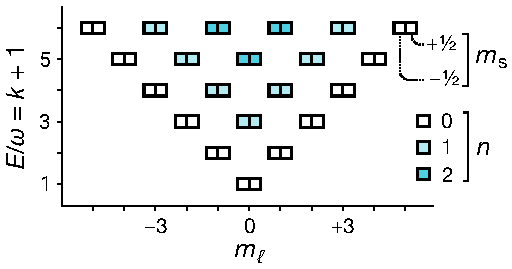
\includegraphics{figures/fig-shell-structure-v2}
  \caption{The 42 lowest single-particle states (the first 5 shells) in the 2D harmonic oscillator basis.  Each box represents a single-particle state arranged by $m_\ell$, $m_{\mathrm{s}}$, and energy, and the up/down arrows indicate the spin of the states.  Within each column, the principal quantum number $n$ increases as one traverses upward.}
  \label{fig:shell-structure}
\end{figure}

The noninteracting part of the many-body Hamiltonian $\hat{H}^{[1]}$ can be reduced to $N$ independent single-particle Hamiltonians each of the form:
\begin{align*}
  \hat{h} = \frac{1}{2} \hat{\bm{\nabla}}^2 + \frac{1}{2} \omega^2 \hat{\bm{r}}^2
\end{align*}
Therefore, solving the noninteracting many-body problem amounts to solving the single-particle Schr\"odinger equation
\begin{align*}
  \hat{h} |p\rangle = \varepsilon_p |p\rangle
\end{align*}
where $p$ is an unknown tuple of quantum numbers.  In Cartesian coordinates, the two-dimensional harmonic oscillator is trivially reducible to the well-known one-dimensional problem.  However, to exploit the circular symmetry, we prefer to use Fock-Darwin states, which are written in polar coordinates $\bm{r} = (\rho, \varphi)$.  Such states have the computationally useful property of conserving orbital angular momentum $\hat{L}_{\mathrm{z}} \equiv -\mathrm{i} \partial / (\partial \varphi)$.

The Fock-Darwin wave functions can be decomposed into radial and angular components,\cite[Appx.\ A]{lohne2010coupled}
\begin{align}
  F_{n, m_\ell}(\rho, \varphi) &\equiv \sqrt\omega R_{n, |m_\ell|}(\sqrt \omega \rho) A_{m_\ell}(\varphi) \label{eq:fockdarwin} \\
  R_{n, m}(\varrho) &\equiv \sqrt{\frac{2 \cdot n!}{(n + m)!}} \mathrm{e}^{-\varrho^2 / 2} \varrho^m L_n^{(m)}(\varrho^2) \notag \\
  A_{m_\ell}(\varphi) &\equiv \frac{1}{\sqrt{2 \pi}} \mathrm{e}^{\mathrm{i} m_\ell \varphi} \notag
\end{align}
where $L_n^{(\alpha)}$ denotes the (generalized) Laguerre polynomial \cite[\S 18.3]{NIST:DLMF} of degree $n$ and parameter $\alpha$,
\begin{align*}
  L_n^{(\alpha)}(u) = \frac{1}{n!} u^{-\alpha} \mathrm{e}^u \frac{\mathrm{d}^n}{\mathrm{d} u^n} (\mathrm{e}^{-u} u^{\alpha + n})
\end{align*}
The states are labeled by two quantum numbers: the principal quantum number $n \in \{0, 1, 2, \ldots\}$ and orbital angular momentum projection $m_\ell \in \mathbb \{\ldots, 2, -1, 0, 1, 2, \ldots\}$.  For a wave function, $n$ indicates the degree of the Laguerre polynomial, whereas $m_\ell$ is simply the eigenvalue of $\hat{L}_{\mathrm{z}}$.

Since electrons are spin-$1/2$ fermions, they can occupy either of the two possible spin states $\chi_{-1/2}$ or $\chi_{+1/2}$.  Thus, every single-particle basis state $| (n, m_\ell, m_{\mathrm{s}}) \rangle$ contains both a spatial component \eqref{eq:fockdarwin} and a spin component,
\begin{align} \label{eq:singleparticlestate}
  \langle (\rho, \varphi), m_{\mathrm{s}}' | (n, m_\ell, m_{\mathrm{s}}) \rangle \equiv F_{n, m_\ell}(\rho, \varphi) \delta_{m_{\mathrm{s}}^{}, m_{\mathrm{s}}'}
\end{align}
Here we have introduced spin projection $m_{\mathrm{s}} \in \bigl\{-1/2, +1/2\bigr\}$ as the third quantum number and $\delta_{p, q}$ to denote the Kronecker delta..

The energy of the single-particle state $| (n, m_\ell, m_{\mathrm{s}}) \rangle$ is given by
\begin{align} \label{eq:energysingleparticlestate}
  \varepsilon_{n, m_\ell, m_{\mathrm{s}}} \equiv (2 n + |m_\ell| + 1) \omega
\end{align}
The energies are degenerate with respect to the spin projection $m_{\mathrm{s}}$ as our Hamiltonian $\hat{h}$ does not distinguish between them.  Additionally, they are degenerate with respect to the nonnegative integer
\begin{align} \label{eq:shell_index}
  k \equiv 2 n + |m_\ell|
\end{align}
which we conveniently call the \textit{shell index} as it labels each shell starting from zero.  The shells are equidistant with an energy spacing equal to the frequency $\omega$.

Returning to the many-body Hamiltonian $\hat{H}^{[1]}$, we can use the Slater determinant construction to build an $N$-particle eigenstate $|p_1, \ldots, p_N\rangle$ of the many-body Hamiltonian $\hat{H}^{[1]}$ from an arbitrary choice of $N$ single-particle eigenstates $|p_1\rangle, \ldots, |p_N\rangle$ from \eqref{eq:singleparticlestate}, where $p$ is an abbreviation for the triplet $(n, m_\ell, m_{\mathrm{s}})$.  Note that a Slater determinant $|p_1, \ldots, p_N\rangle$ is not merely a product of the single-particle states, but an antisymmetrized sum over all possible products,
\begin{align*}
  \langle \bm{r}_1, \ldots, \bm{r}_N | p_1, \ldots, p_N \rangle \equiv
  \frac{1}{\sqrt{N}} \left|
  \begin{matrix}
    \langle \bm{r}_1 | p_1 \rangle & \cdots & \langle \bm{r}_1 | p_N \rangle \\
    \vdots & \ddots & \vdots \\
    \langle \bm{r}_N | p_1 \rangle & \cdots & \langle \bm{r}_N | p_N \rangle \\
  \end{matrix}
  \right|
\end{align*}
The Slater determinant $|p_1, \ldots, p_N\rangle$ is said to \textit{occupy} the states $|p_1\rangle, \ldots, |p_N\rangle$.  By construction, Slater determinants satisfy the Pauli exclusion principle, ensuring that the exchange of any two particles is equivalent to a reversal in the sign of the many-body wave function.

The energy of a Slater determinant is given by a sum over the occupied single-particle energies,
\begin{align*}
  \hat{H}^{[1]} | p_1, \ldots, p_N \rangle = (\varepsilon_{p_1} + \cdots + \varepsilon_{p_N}) | p_1, \ldots, p_N \rangle
\end{align*}
It is possible for Slater determinants occupying different sets of single-particle states to be degenerate in energy.  This is possible even for ground states of $\hat{H}^{[1]}$.  However, if the number of particles $N$ satisfies $N = K_{\mathrm{F}} (K_{\mathrm{F}} + 1)$ for some nonnegative integer $K_{\mathrm{F}}$, there would be just enough particles to form a closed-shell Slater determinant, leading to a unique, well-isolated ground state.  The values of $N$ at which this occurs are said to be \textit{magic numbers}.  We call $K_{\mathrm{F}}$ the \textit{number of filled shells} (or ``Fermi level'').  In particular, a single-particle state is occupied in the ground state Slater determinant if and only $k < K_{\mathrm{F}}$, where $k$ is the shell index of the single-particle state as defined in \eqref{eq:shell_index}.

Currently, the Hamiltonian $\hat{H}$ is defined for a fixed number of particles $N$.  Through the formalism of second quantization, the many-body machinery can be made agnostic to number of particles, in analogy to quantum field theory.  Instead of considering the Hilbert space for exactly $N$ particles, we combine every space with $N = 0, 1, 2, \ldots$ particles into a combined Hilbert space called the Fock space.  To establish relationships between states with differing number of particles, we introduce the \textit{field operators} $\hat{a}_p^\dagger$ and $\hat{a}_p$ to increment and decrement the number of particles in a state, respectively.  The linear operator $\hat{a}_p^\dagger$ is known as \textit{creation operator} for the single-particle state $p$.  Its action on an arbitrary Slater determinant is defined as:
\begin{align*}
  \hat a_p^\dagger |p'_1, \ldots, p'_N\rangle =
  |p, p'_1, \ldots, p'_N\rangle
\end{align*}
Informally, it is said to \textit{create} a particle in the state $p$.  If $p$ coincides with any of the existing $p'_1, \ldots, p'_N$, then antisymmetrization would collapse the state to the number $0$, an invalid state.  The Hermitian conjugate of $\hat{a}_p^\dagger$ is $\hat{a}_p$, which known as the \textit{annihilation operator} for the state $p$.  By analogy, its action is to remove the state $p$ from a Slater determinant, or collapse it to the number $0$ if the state $p$ was not occupied in the Slater determinant.

From here, one can show that Slater determinants themselves can be built directly from the the unique \textit{vacuum state} $|\rangle$ with no particles ($N = 0$):
\begin{align*}
  |p_1, \ldots, p_N\rangle =
  \hat a_{p_1}^\dagger \cdots \hat a_{p_N}^\dagger |\rangle
\end{align*}
To properly describe fermions, the field operators $\hat a_p$ and $\hat a_p^\dagger$ must satisfy the anticommutation relations that encode the Pauli principle,
\begin{align*}
  &\{\hat a_p, \hat a_q\} = \{\hat a_p^\dagger, \hat a_q^\dagger\} = 0 &
  &\{\hat a_p, \hat a_q^\dagger\} = \delta_{p, q}
\end{align*}

In second quantization, the one- and two-body Hamiltonian operators $H^{[1]}$ and $\hat{H}^{[2]}$ from \eqref{eq:onetwobodyhamiltonian} can be rewritten as\footnote{The peculiar ordering of $\hat a_s \hat a_r$ here is not a typographical error.}
\begin{align} \label{eq:second_quantized_hamiltonian}
  \hat H^{[1]} &= \sum_{p, q} \langle p | \hat{H}^{[1]} | q \rangle \hat a_p^\dagger \hat a_q^{} &
  \hat{H}^{[2]} &= \frac{1}{4} \sum_{p, q, r, s} \langle p, q | \hat{H}^{[2]} | r, s \rangle \hat a_p^\dagger \hat a_q^\dagger \hat a_s^{} \hat a_r^{}
\end{align}
where the numeric coefficients $\langle p | \hat{H}^{[1]} | q \rangle$ and $\langle p, q | \hat{H}^{[2]} | r, s \rangle$ are known as \textit{matrix elements} and fully characterize the two operators in the basis.  In this paper, we use the letters $p, q, r, s, t, \ldots$ to label arbitrary single-particle \textit{states} in the basis.  For the harmonic oscillator basis, labels such as $p$ can be considered abbreviations for triplets of the form $(n, m_\ell, m_{\mathrm{s}})$.  A summation such as $\sum_p$ is then understood as a summation over every single-particle basis state $p$.  This is not to be confused with summations such as $\sum_j$ from \eqref{eq:onetwobodyhamiltonian}, which contains a label $j$ denoting an arbitrary \textit{particle}.  We thus see another benefit with second quantization: the Hamiltonian representation makes no attempt to distinguish particles at all, as expected for particles with quantum statistics.

The complete Hamiltonian is given by the sum
\begin{align}
  \hat{H} = \sum_{p, q} \langle p | \hat{H}^{[1]} | q \rangle \hat{a}_p^\dagger \hat{a}_q + \frac{1}{4} \sum_{p, q, r, s} \langle p, q | \hat{H}^{[2]} | r, s \rangle \hat{a}_p^\dagger \hat{a}_q^\dagger \hat{a}_s \hat{a}_r  \label{eq:vacuumhamiltonian}
\end{align}
Due to antisymmetry of Slater determinants, we have the property that exchanging either $p$ with $q$ or $r$ with $s$ reverses the sign of $\langle p, q | \hat{H}^{[2]} | r, s \rangle$, leading to a 4-fold symmetry that must be canceled out by the $1/4$ factor in front of the summation in \eqref{eq:vacuumhamiltonian}.  For this reason, the two-body matrix element $\langle p, q | \hat{H}^{[2]} | r, s \rangle$ is commonly referred to as the \emph{antisymmetrized} matrix element.  This is not to be confused with the (non-antisymmetric) interaction integral,
\begin{align} \label{eq:interactionintegral}
  v_{p_1, p_2, p_3, p_4} \equiv \int \langle p_1 | \bm{r} \rangle \langle p_2 | \bm{r}' \rangle v(\bm r, \bm r') \langle \bm{r} | p_3 \rangle \langle \bm{r}' | p_4 \rangle \D \bm{r} \D \bm{r}'
\end{align}
This object only has a 2-fold symmetry: $v_{p_1, p_2, p_3, p_4} = v_{p_2, p_1, p_4, p_3}$.  The antisymmetrized matrix element are related to the interaction integral via
\begin{align} \label{eq:antisymmetricmatrixelement}
  \langle p, q | \hat{H}^{[2]} | r, s \rangle = v_{p, q, r, s} - v_{p, q, s, r}
\end{align}

With the basic formalism and notation established along with the system of interest, we may begin to discuss the various techniques to solve the full many-body problem.  The principal difficulty stems from the fact that, due to the presence of interactions, the exact solution is in general \emph{not} a single Slater determinant built from the single-particle states.  Hence, it is not possible to trivially reduce the problem to that of a single particle as we had done previously.

However, if we assume the interaction alters the behavior of the system only mildly, we can use a Slater determinant of the noninteracting system as a starting point and then apply various methods to improve the accuracy of the solution.  This is a general strategy for many of the many-body methods that we shall describe.

\subsection{Hartree--Fock method}
\label{subsec:HartreeFockmethod}

One of the simplest numerical corrections that could be applied to the initial guess is that of the Hartree--Fock (HF) method.  Using the variational principle, one can compute an approximate ground state $\Phi$ by minimizing the energy expectation value
\begin{align} \label{eq:hfexpectation}
  E_{\Phi} \equiv \langle \Phi | \hat H | \Phi \rangle
\end{align}
with respect to $|\Phi\rangle$, subject to the restriction that $|\Phi\rangle$ remains a single Slater determinant constructed from an unknown single-particle basis.  The restriction is what enables the simplicity and efficiency of this method.  We shall denote each unknown single-particle state $|q'\rangle$ by a primed label $q'$.

To perform numerical calculations, we further assume that each unknown state $|q'\rangle$ is built from a linear combination of known states $|p\rangle$, with an unknown matrix of coefficients $\bm C$ defined via the transformation equation
\begin{align*}
  |q'\rangle \equiv \sum_p |p\rangle C_{p, q'}
\end{align*}
This allows the problem to be reduced from an abstract minimization problem \eqref{eq:hfexpectation} to a concrete numerical problem.  The caveat is that the set of known functions be large enough to capture the relevant behavior of the system.

If the interaction is not too strong, it is common to use the single-particle states of the noninteracting Hamiltonian $\hat{H}^{[1]}$ as the set of known states.

To ensure orthonormality of the states, we require there to be as many unknown states $|q'\rangle$ as known states $|p\rangle$, and the coefficient matrix $\bm C$ must be unitary.  These conditions are more strict than necessary, but they greatly simplify the calculations and allow the states $|q'\rangle$ to act as \textit{optimized} inputs for methods beyond HF.  At the end of the calculation, of the set of states $|q'\rangle$ there would exactly $N$ \textit{occupied} states that participate in the optimized Slater determinant $|\Phi\rangle$.  The remaining \textit{unoccupied} states serve as the complementary space into which particles can be excited by the interaction $\hat{H}^{[2]}$ during the post-HF calculation.

The goal then is to find the coefficients $\bm C$ that minimize the energy $E_{\Phi}$, now given by
\begin{align}
  E_{\Phi} &= \sum_i n_i H^{[1] \prime}_{i, i} + \sum_{i, j} n_i n_j H^{[2] \prime}_{i, j, i, j} \label{eq:hfenergy}
\end{align}
where the transformed operators are defined as
\begin{align}
  H^{[1] \prime}_{p, q} &\equiv \sum_{r, s} C_{r, p}^* \langle r | \hat{H}^{[1]} | s \rangle C_{s, q}^{} \label{eq:hftransform1} \\
  H^{[2] \prime}_{p, q, r, s} &\equiv \sum_{t, u, v, w} C_{t, p}^* C_{u, q}^* \langle t, u | \hat{H}^{[2]} | v, w \rangle C_{v, r}^{} C_{w, s}^{} \label{eq:hftransform2}
\end{align}
and $n_p$ is the \textit{occupancy}, defined as
\begin{align}
  n_p \equiv \begin{cases}
    1 & \text{if $p$ is an occupied state in $\Phi$} \\
    0 & \text{if $p$ is an unoccupied state in $\Phi$}
  \end{cases}
\end{align}
We will also use $\bar n_p \equiv 1 - n_p$ as a shorthand for the complement.

With the method of Lagrange multipliers, the minimization problem can be reduced to the solving of a nonlinear equation -- the \textit{Hartree--Fock equation}:
\begin{align} \label{eq:hartreefock}
  \bm{F} \bm{C} = \bm{C} \bm{\varepsilon}
\end{align}
where the \textit{Fock matrix} $\bm F$ is defined as
\begin{align} \label{eq:fock}
  F_{p, q} \equiv \langle p | \hat{H}^{[1]} | q \rangle + \sum_{r, s, i} n_i C_{r, i}^* \langle p, r | \hat{H}^{[2]} | q, s \rangle C_{s, i}^{}
\end{align}
and $\bm{\varepsilon}$ is a vector of Lagrange multipliers: each element $\varepsilon_{q'}$ is associated with a specific single-particle state $|q'\rangle$.

Aside from trivial cases, the HF equation is generally solved using an iterative algorithm.  We begin with an initial guess $\bm{C}^{(i)}$, which is fed into \eqref{eq:fock} to produce the Fock matrix.  This is then used in \eqref{eq:hartreefock}, which leads to a standard eigenvalue problem from which $\bm{C}^{(i + 1)}$ arise as the matrix of eigenvectors and $\bm{\varepsilon}^{(i + 1)}$ as the vector of eigenvalues.  This process can be repeated indefinitely until $\bm{C}$ approaches a fixed point.  While in theory it is possible for the solution to never reach a fixed point, or that it may require a unfeasibly large number of iterations, in practice this naive approach can adequately provide solutions for many cases.  In other cases where it is insufficient, methods such as DIIS, Broyden's method, or even \textit{ad hoc} linear mixing can improve and accelerate convergence greatly.  Therefore, the possibility of slow or non-convergence is generally not a concern in practice.

For the initial guess, we simply use the ground state of our noninteracting Hamiltonian, thus $\bm{C}^{(0)} = \bm{1}$, the identity matrix.  At each iteration, we calculate the sum of the Lagrange multipliers $\bm{\varepsilon}$ as a diagnostic for convergence: as the iteration approaches convergence, the change in the sum per iteration should decrease rapidly.

Since HF restricts the ground state to merely a single Slater determinant of single-particle states, it cannot provide an exact solution to a problem where multi-particle correlations are present even if the single-particle basis is not truncated (infinite in size).  The discrepancy between the Hartree--Fock energy and the exact ground state energy is often referred to as the \textit{correlation energy}, by definition.  The focus of post-HF methods such as IM-SRG or coupled cluster is to add corrections beyond mean-field approximations such as HF.

To make use of the HF solution as the reference state for future calculations, we transform the operators via \eqref{eq:hftransform1} and \eqref{eq:hftransform2}.  Therefore, the post-HF methods described in the next few sections generally use the transformed operators $\hat{H}^{[1] \prime}$ and $\hat{H}^{[2] \prime}$ as inputs.  However, we will not annotate them with the prime symbols as the methods are generic and can be applied to any reference state, whether optimized by HF or not.

\subsection{The IM-SRG method}
\label{subsec:imsrgmethod}

\subsubsection{Similarity renormalization group in free space}
\label{subsubsec:srgmethods}

The central theme of similarity renormalization group (SRG) methods is the application of a continuous sequence of unitary transformations on the Hamiltonian to evolve it into a band- or block-diagonal form.  This allows the decoupling of a small, designated \textit{model space} from its larger complementary space.  The problem can thus be truncated to the small model space while preserving a large amount of information about the system.

The sequence of transformations is parameterized by a continuous variable $s$ known as the \textit{flow parameter}.  Without loss of generality, we can define $s = 0$ to be the beginning of this sequence, thus $\hat{H}(0)$ is simply the original Hamiltonian.  At any value of $s$, the evolving Hamiltonian $\hat{H}(s)$ is related to the original Hamiltonian by
\begin{align*}
  \hat{H}(s) \equiv \hat{U}(s) \hat{H}(0) \hat{U}^\dagger(s)
\end{align*}
where $U(s)$ is a unitary operator that describes the product of all such
transformations since $s = 0$.  Taking the derivative with respect to $s$, we obtain:
\begin{align*}
  \frac{\D}{\D s} \hat{H}(s) = \frac{\D \hat{U}(s)}{\D s} \hat{H}(0) \hat{U}^\dagger(s) + \hat{U}(s) \hat{H}(0) \frac{\D \hat{U}^\dagger (s)}{\D s}
\end{align*}
If we define an operator $\hat{\eta}(s)$ as
\begin{align} \label{eq:etadefinition}
  \hat{\eta}(s) \equiv \frac{\D \hat{U}(s)}{\D s} \hat{U}^\dagger(s)
\end{align}
we find that it is antihermitian as a result of the unitarity of $\hat{U}(s)$:
\begin{align*}
  \hat{\eta}(s) + \hat{\eta}^\dagger(s)
  = \frac{\D}{\D s} \left(\hat{U}(s) \hat{U}^\dagger(s)\right)
  = 0
\end{align*}
From this property we can derive a differential equation known as the \textit{SRG flow equation}:
\begin{align} \label{eq:imsrgode}
  \frac{\D \hat{H}(s)}{\D s} = [\hat{\eta}(s), \hat{H}(s)]
\end{align}
The equation allows $\hat{H}(s)$ to be evaluated without explicitly constructing the full transformation $\hat U(s)$.  The focus is instead shifted to the operator $\hat \eta(s)$, the \textit{generator} of the transformation.  When $\hat \eta(s)$ is \emph{multiplicatively} integrated (\textit{product integral}), the full unitary transformation $\hat U(s)$ is recovered:
\begin{align} \label{eq:etaintegral}
  \hat U(s')
  = \lim_{\Delta s \to 0} \prod_{i = 1}^n \mathrm{e}^{\hat{\eta}(s_i) \Delta s}
\end{align}
where $s_i \equiv i \Delta s$, $n \equiv \lfloor s' / \Delta s \rfloor$, and $\lfloor x \rfloor$ denotes the \textit{floor} of $x$.  This is the formal solution to the linear differential equation \ref{eq:etadefinition}.  The product integral in \ref{eq:etaintegral} may also be reinterpreted as \textit{$s$-ordering} \cite[\S 6.1]{reimann2013quantum} in analogy to time-ordering from quantum field theory.

The power of SRG methods lies in the flexibility of the generator $\hat{\eta}$, which is usually chosen in an $s$-dependent manner.  In particular, it is often dependent on the evolving Hamiltonian $\hat{H}(s)$.  The operator $\hat{\eta}$ determines which parts of the Hamiltonian matrix would become suppressed by the evolution, which are usually considered ``off-diagonal'' in an abstract sense.  The ``off-diagonal'' parts could be elements far away from the matrix diagonal, in which case the evolution drives the matrix towards a band-diagonal form.  Or, the ``off-diagonal'' parts could be elements that couple the ground state from the excited state, in which case the evolution drives the matrix towards a block-diagonal form that isolates the ground state.  Or, the ``off-diagonal'' could be literally the elements that do not lie on the diagonal, in which case the evolution would simply diagonalize the Hamiltonian.  Through different choices of $\hat{\eta}$, the SRG evolution can be controlled and adapted to the features of a particular problem.

\subsubsection{Evolving the flow equation in medium}

The SRG flow equation \eqref{eq:imsrgode} can be solved in the second quantization formalism described in Section \ref{subsec:modelHamiltonian}, where field operators are defined with respect to the physical vacuum state.  However, since the basis of a many-body problem grows factorially with the number of particles and the size of the model space, the applicability of the naive (free-space) SRG method is restricted to comparatively small systems.  A more practical approach is to perform the evolution \textit{in medium}, i.e.\ using a many-body Slater determinant as a reference \cite{kehrein2006flow}.  This gives rise to the IM-SRG method.

The second-quantized operators in \eqref{eq:second_quantized_hamiltonian} are constructed with respect to the vacuum state in the sense that their operator strings $\hat{a}_p^\dagger \hat{a}_q$ and $\hat{a}_p^\dagger \hat{a}_q^\dagger \hat{a}_s \hat{a}_r$ both have expectation values of zero in vacuum:
\begin{align*}
&\bra{} \hat{a}_p^\dagger \hat{a}_q \ket{} = 0 &
&\bra{} \hat{a}_p^\dagger \hat{a}_q^\dagger \hat{a}_s \hat{a}_r \ket{} = 0
\end{align*}
They are said to be \emph{normal-ordered} with respect to the vacuum state $\ket{}$.  It is possible to be normal-ordered with respect to a different state, however.  Suppose we have a Slater determinant $\Phi$ with $N$ occupied states:
\begin{align*}
  \ket{\Phi} \equiv \ket{i_1, i_2, \ldots, i_N}
\end{align*}
where $\{i_1, i_2, \ldots, i_N\}$ is a set of $N$ indices that label the occupied states.  One can define a set of \textit{quasiparticle field operators} $\hat b$ and $\hat b^\dagger$ that obey the same anticommutation relations as the $\hat a$ operators:
\begin{align*}
  \hat b_p \equiv \bar n_p \hat a_{p} + n_p \hat a_{p}^\dagger
\end{align*}
The quasiparticle field operators treat the \textit{reference state} $\ket{\Phi}$ as their ``vacuum'' state (\textit{Fermi vaccuum}), even though it is not the true \emph{physical} vacuum state.  As before, it is possible to construct arbitrary Slater determinants by applying quasiparticle operators to the reference state:
\begin{align}
  \ket{\Phi_{p_1, \ldots, p_k}} \equiv \hat{b}^\dagger_{p_1} \cdots \hat{b}^\dagger_{p_k} \ket{\Phi}
  \label{eq:quasisd}
\end{align}
If $p$ is an unoccupied state, then applying $\hat{b}_p^\dagger$ creates a particle exactly like $\hat{a}_p^\dagger$.  However, if $p$ is an occupied state, then applying $\hat{b}_p^\dagger$ destroys an existing particle in $\Phi$ or, equivalently, creates a \textit{hole} state.  The set of labels $\{p_1, \ldots, p_k\}$ may contain up to $N$ hole states and as many particle states as the basis allows for (minus the ones that are already hole states).  One can classify the state $\Phi_{p_1, \ldots, p_k}$ as an $N_{\text{p}}$-particle-$N_{\text{h}}$-hole state, meaning that it contains $N_{\text{p}}$ labels that denote unoccupied states and $N_{\text{h}}$ labels that denote occupied states.  If $N_{\text{p}} = N_{\text{h}}$, the Slater determinant contains the same number of physical particles as the reference state.  The ``$N_{\text{p}}$-particle-$N_{\text{h}}$-hole'' classification gives a crude sense of how distant a state is from the reference state, which can be exploited by many-body theories.

We may then define \emph{normal ordering with respect to the reference state} $\Phi$, a notational device that reorders a string of operators such that every quasiparticle creation operator appears before a quasiparticle annihilation operator, while also accounting for the sign.  Each exchange of operators must incur a change in sign -- mathematically this is just the \textit{sign} of the permutation that reorders the operators.  A simple example would be the normal ordering of a pair of field operators such as:
\begin{align*}
  \normord{\hat{b}_p^{} \hat{b}_q^\dagger} =
  -\hat{b}_q^\dagger \hat{b}_p^{}
\end{align*}
Here, we denote normal ordering of an operator string with respect to $\Phi$ by a enclosing pair of colons.  The expectation value of a normal ordered string of operators with respect to $\Phi$ is guaranteed to vanish:
\begin{align*}
&\bra{\Phi} \hat{b}_p^\dagger \hat{b}_q^{} \ket{\Phi} = 0 &
&\bra{\Phi} \hat{b}_p^\dagger \hat{b}_q^\dagger \hat{b}_s^{} \hat{b}_r^{} \ket{\Phi} = 0
\end{align*}
The normal ordering of the quasiparticle field operators is straightforward to compute.  What is more interesting is the normal ordering of the physical field operators $\hat a$ and $\hat a^\dagger$ with respect to $|\Phi\rangle$:
\begin{align*}
  \normord{\hat{a}_p^\dagger \hat{a}_q^{}} &=
  \hat{a}_p^\dagger \hat{a}_q^{} - n_p^{} \delta_{p, q}^{}
\end{align*}
The normal ordering notation thus provides a concise way of expressing the right-hand side.  In this new notation, we can rewrite the Hamiltonian $\hat H = \hat{H}^{[1]} + \hat{H}^{[2]}$ in its \emph{normal-ordered representation}:
\begin{align}
  \hat{H} = H^{[0]} + \sum_{p, q} H^{[1]}_{p, q} \normord{\hat{a}_p^\dagger \hat{a}_q^{}} + \frac{1}{4} \sum_{p, q, r, s} H^{[2]}_{p, q, r, s} \normord{\hat{a}_p^\dagger \hat{a}_q^\dagger \hat{a}_s^{} \hat{a}_r^{}}
  \label{eq:normordhamiltonian}
\end{align}
where
\begin{align*}
  H^{[0]} &\equiv \sum_{i} n_i \langle i | \hat{H}^{[1]} | i \rangle + \frac{1}{2} \sum_{i, j} n_i n_j \langle i, j | \hat{H}^{[2]} | i , j \rangle \\
  H^{[1]}_{p, q} &\equiv \langle p | \hat{H}^{[1]} | q \rangle + \sum_{i} n_i \langle p, i | \hat{H}^{[2]} | q, i \rangle \\
  H^{[2]}_{p, q, r, s} &\equiv \langle p, q | \hat{H}^{[2]} | r, s \rangle \\
\end{align*}
If $\Phi$ is a state optimized by the HF method, then $H^{[0]}$ is simply the HF energy $E_\Phi$ and $H^{[1]}_{p, q}$ is the Fock matrix $F_{p, q}$.  The operator $\hat H$ in \eqref{eq:normordhamiltonian} is completely equivalent to $\hat H$ in \eqref{eq:vacuumhamiltonian}.  The only difference is that the meaning of a ``$k$-body operator'' has been redefined with respect to the reference state $\Phi$ rather than vacuum state $\ket{}$, causing matrix elements to be reshuffled among the $k$-body operators.  Where this makes a critical difference is when the operator expressions are \emph{truncated}, i.e.\ some $k$-body operators may be discarded from the computation for efficiency reasons.  Normal-ordering can drastically alter the importance of the $k$-body operators with respect to each other.

Higher-body operators arise from integrating the flow equations (\ref{eq:imsrgode}), which is one of the major challenges of the SRG method.  With each evaluation of the commutator, the Hamiltonian gains terms of higher order, and these induced contributions will in subsequent integration steps feed back into terms of lower order.  Thus, the higher-body contributions are not irrelevant to the final solution even if only the ground state energy (zero-body component) is of interest.

Computationally, higher-body terms rapidly become unfeasible to handle: the amount of memory required to store a $k$-body operator is grows exponentially with $k$.  Moreover, the flow equations are capable of generating an infinite number of higher-body terms as the Hamiltonian evolves.  Thus, to make the method tractable, the IM-SRG flow equations must be closed by truncating the equations to a finite order.

In this paper, we truncate both $\hat{H}$ and $\hat{\eta}$ at the two-body level, leading to an approach known as IM-SRG(2).  This normal-ordered two-body approximation appears to be sufficient in many cases and has yielded excellent results for several nuclei \cite{PhysRevLett.106.222502,PhysRevLett.109.052501,IMSRG}.

Note that the loss of three- and higher-body terms (\textit{operator truncation}) is only one out of the two sources of error in this method.  The other source of error is due to the \textit{basis truncation}, a concern for any method that relies on a finite single-particle basis such as IM-SRG.  The latter can be reduced by increasing the size of the basis at the expense of greater computational effort, albeit the cost increases much less rapidly in this direction.  In IM-SRG the CPU cost is polynomial with respect to $N_{\mathrm{b}}$, the number of states in the single-particle basis.  For IM-SRG(2) in particular, the CPU cost scales roughly as $\mathcal{O}(N_{\mathrm{b}}^6)$.

With the operator truncation, the generator $\hat{\eta}$ can be written as a generic 2-body operator:
\begin{align*}
\hat{\eta} = \sum_{p, q} \eta_{p, q}^{[1]} \normord{\hat a_p^\dagger \hat a_q} +
\frac{1}{4} \sum_{p, q, r, s}\eta_{p, q, r, s}^{[2]} \normord{\hat a_p^\dagger \hat a_q^\dagger \hat a_s \hat a_r}
\end{align*}
where $\eta_{p, q}^{[1]}$ and $ \eta_{p, q, r, s}^{[2]}$ respectively are its one- and two-body matrix elements normal ordered with respect to $\Phi$, subject to the antihermittivity constraint.

By expanding the commutator in \eqref{eq:imsrgode} and discarding the three-body term, we obtain the matrix-element form of the IM-SRG(2) flow equation:
\begin{align}
    \frac{\D H^{[k]}}{\D s} = C^{[k]}(\eta, H) \label{eq:flowmxe}
\end{align}
where
\begin{align}
  C^{[k]}(A, B) &\equiv 2 \mathcal{A}_{A, B} D^{[k]}(A, B) \text{ for any $k$, $A$, $B$} \label{eq:commutmxe} \\
  \mathcal{A}_{x, y} f(x, y) &\equiv \frac{1}{2} \bigl(f(x, y) - f(y, x)\bigr) \text{ for any $x$, $y$, $f$}
\end{align}
\begin{align}
  D^{[0]}(A, B)
  &\equiv
    \sum_{i, a} n_i \bar{n}_a A^{[1]}_{i, a} B^{[1]}_{a, i}
    + \frac{1}{4} \sum_{i, j, a, b} n_i n_j \bar{n}_a \bar{n}_b A^{[2]}_{i, j, a, b} B^{[2]}_{a, b, i, j}
    \label{eq:flow0} \\
  D^{[1]}_{p, q}(A, B)
  &\equiv
    \sum_{r} A^{[1]}_{p, r} B^{[1]}_{r, q}
    - \frac{1}{2} \sum_{i, j, a} n_i n_j \bar{n}_a A^{[2]}_{i, j, a, q} B^{[2]}_{a, p, i, j}
    + \frac{1}{2} \sum_{i, a, b} n_i \bar{n}_a \bar{n}_b A^{[2]}_{i, p, a, b} B^{[2]}_{a, b, i, q}
    \notag \\
  &\hphantom{=}
    + \sum_{i, a} n_i \bar{n}_a \left(
    A^{[1]}_{i, a} B^{[2]}_{a, p, i, q}
    + A^{[2]}_{i, p, a, q} B^{[1]}_{a, i}
    \right)
    \label{eq:flow1} \\
  D^{[2]}_{p, q, r, s}(A, B)
  &\equiv
    \tilde{\mathcal{A}}_{p, q} \tilde{\mathcal{A}}_{r, s}
    \sum_{i, a} n_i \bar{n}_a A^{[2]}_{i, p, a, r} B^{[2]}_{a, q, i, s}
    \notag \\
  &\hphantom{=}
    + \frac{1}{2} \sum_{i, j} n_i n_j A^{[2]}_{i, j, r, s} B^{[2]}_{p, q, i, j}
    + \frac{1}{2} \sum_{a, b} \bar{n}_a \bar{n}_b A^{[2]}_{p, q, a, b} B^{[2]}_{a, b, r, s}
    \notag \\
  &\hphantom{=}
    + \sum_{t} \left(
    \tilde{\mathcal{A}}_{p, q} A^{[1]}_{q, t} B^{[2]}_{p, t, r, s}
    + \tilde{\mathcal{A}}_{r, s} A^{[2]}_{p, q, r, t} B^{[1]}_{t, s}
    \right)
    \label{eq:flow2}
\end{align}

\begin{figure}
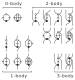
\includegraphics{fig-diagrams-imsrg}
\caption{Diagrammatic representation of $D^{[k]}(\circ, \bullet)$ of \eqref{eq:flow0}, \eqref{eq:flow1}, and \eqref{eq:flow2}, where open circles represent $A$ and filled circles represent $B$.  The two-body vertices are implicitly antisymmetric (i.e.\ \textit{Hugenholtz diagrams} \cite{HUGENHOLTZ1957481}, as described in \cite{shavitt2009many} \S 4.4.3).  Internal directed lines (bound/dummy indices) that point upward denote summations over unoccupied states, whereas lines that point downward denote summations over occupied states.  External undirected lines denote unconstrained free indices.  In IM-SRG(2), the three-body diagrams are not included.}
\label{fig:diagrams-imsrg}
\end{figure}

The equations can be derived directly from the anticommutation relations of the field operators, but it is more convenient to use Wick's theorem \cite{PhysRev.80.268} or, even more efficiently, diagrammatic techniques \cite{shavitt2009many} to arrive at the results.  In particular, Figure \ref{fig:diagrams-imsrg} shows the diagrammatic form of \eqref{eq:flow0}, \eqref{eq:flow1}, and \eqref{eq:flow2}.

The commutator in the flow equations \eqref{eq:imsrgode} ensures that the evolved state $\hat U(s) \ket{\Phi}$ consists of \emph{linked diagrams} only \cite{shavitt2009many}.  This indicates that IM-SRG is a size-extensive \cite{ISI:A1981MN73700014} method by construction, even if the operators are truncated.

An accurate and robust ODE solver is required to solve \eqref{eq:imsrgode}.  In particular, the solver must be capable of handling the stiffness that often arises in such problems.  For our numerical experiments, we used a high-order ODE solver algorithm by L.\ F.\ Shampine and M.\ K.\ Gordon \cite{shampine1975computer}, which is a multistep method based on the implicit Adams predictor-corrector formulas.  Its source code is freely available \cite{odesolver}.

Through the flow equation and with an appropriate choice of the generator $\hat{\eta}$, the evolved state $\hat U(s) \ket{\Phi}$ will gradually approach a more ``diagonal'' form.  If the ``diagonal'' form decouples the ground state from the excited states, then $\hat U(\infty) \ket{\Phi}$ would yield the exact ground state solution of the problem if no operator or basis truncations are made.  In particular, $H^{[0]}(\infty)$ would be the exact ground state energy.

The original choice of generator suggested by Wegner \cite{Wegner200177} reads
\begin{align*}
  \hat{\eta}^{\text{Wg}}
  = [\hat{H}^{\text{d}}, \hat{H} - \hat{H}^{\text{d}}]
  = [\hat{H}^{\text{d}}, \hat{H}]
\end{align*}
where $\hat{H}^{\text{d}}$ denotes the ``diagonal'' part of the Hamiltonian and $\hat{H} - \hat{H}^{\text{d}}$ denotes the ``off-diagonal'' part.  This is in the abstract sense described at the end of Section \ref{subsubsec:srgmethods}.

Since $\hat{\eta}^{\text{Wg}}$ is a commutator between two Hermitian operators, it is antihermitian as required for a generator.  Additionally, it can be shown that the commutator has the property of suppressing off-diagonal matrix elements as the state evolves via the flow equation \cite{kehrein2006flow}, as we would like.  Matrix elements ``far'' from the diagonal -- i.e.\ where the Hamiltonian couples states with large energy differences -- are suppressed much faster than those ``close'' to the diagonal.

Apart from Wegner's generator, there exist several other ones in literature. One choice, proposed by White \cite{White:cond-mat0201346}, makes numerical approaches much more efficient.  The problem with the Wegner generator is the widely varying decaying speeds of the Hamiltonian matrix elements.  Terms with large energy separations from the ground state are suppressed initially, followed by those with smaller energy separations.  This leads to stiffness in the flow equation, leading to numerical difficulties in solving the set of coupled differential equations.

The White generator takes an alternative approach, which is well suited for problems where one is mainly interested in the ground state of a system.  Firstly, instead of driving all off-diagonal elements of the Hamiltonian to zero, the generator focuses exclusively on those ones that are coupled to the reference state $\Phi$ so as to decouple the reference state from the remaining Hamiltonian.  This reduces the amount of change done to the Hamiltonian, reducing the accuracy lost from the operator truncation.  Secondly, the rate of decay in Hamiltonian matrix elements are approximately normalized by dividing the generator matrix elements by an appropriate factor.  This ensures that the affected elements decay at approximately the same rate, reducing the stiffness of the flow equations.

The White generator is explicitly constructed the following way \cite{PhysRevLett.106.222502,White:cond-mat0201346}.  Let
\begin{align*}
\hat{\eta}^{\text{Wh}} &\equiv \hat{\eta}' - \hat{\eta}'{}^\dagger
\end{align*}
where
\begin{align*}
\eta^{\prime [1]}_{a, i} &\equiv \frac{\bar{n}_a n_i H^{[1]}_{a, i}}{\tilde{\Delta}^{[1]}_{a, i}} &
\eta^{\prime [2]}_{a, b, i, j} &\equiv \frac{\bar{n}_a \bar{n}_b n_i n_j H^{[2]}_{a, b, i, j}}{\tilde{\Delta}^{[2]}_{a, b, i, j}}
\end{align*}
and the Epstein--Nesbet denominators $\tilde{\Delta}$ are defined as
\begin{align}
\tilde{\Delta}^{[1]}_{a, i} &\equiv \Delta_{\{a\}, \{i\}} - H^{[2]}_{a, i, a, i} \notag \\
\tilde{\Delta}^{[2]}_{a, b, i, j} &\equiv \Delta_{\{a, b\}, \{i, j\}} + w_{a, b, i, j} \notag \\
\Delta^{[2]}_{P_1, P_2} &\equiv \sum_{p_1 \in P_1} H^{[1]}_{p_1, p_1} - \sum_{p_2 \in P_2} H^{[1]}_{p_2, p_2} \label{eq:moellerplessetdenominator} \\
w_{a, b, i, j}
  &\equiv H^{[2]}_{a, b, a, b} - H^{[2]}_{a, i, a, i} - H^{[2]}_{b, i, b, i} \notag \\
  &\qquad + H^{[2]}_{i, j, i, j} - H^{[2]}_{a, j, a, j} - H^{[2]}_{b, j, b, j} \notag
\end{align}
Some literature use the M\o ller--Plesset denominators $\Delta$ instead, leading to a slightly different variant of the White generator.

Compared to the Wegner generator, where the derivatives of the final flow equations contain cubes of the Hamiltonian matrix elements (i.e.\ each term contains a product of 3 one-body and/or two-body matrix elements), the elements in White generators contribute only linearly.  This reduces the stiffness in the differential equation, providing a net increase in computational efficiency as stiff ODE solvers tend to be slower and consume more memory.

\subsection{Coupled-cluster theory}
\label{subsec:cctheory}

Coupled-cluster theory is based on expressing the A-particle correlated wave function using the exponential ansatz, $\ket{\Psi} = e^{\hat{T}}\ket{\Phi}$.  The cluster operator $\hat{T} = \hat{T}_{1} + \hat{T}_{2} + ... + \hat{T}_{A}$, is composed of $N$-particle $N$-hole excitation operators, $\hat{T}_{N}$,
\begin{equation}\label{eq:cc_amps}
\hat{T}_{N} = \left( \frac{1}{N!} \right)^{2}\sum\limits_{\substack{a_{1} \cdots a_{N} \\ i_{1} \cdots i_{N}}} \bar{n}_{a_{1}} \cdots \bar{n}_{a_{N}} n_{i_{1}} \cdots n_{i_{N}}\ t_{a_{1} \cdots a_{N}, i_{1} \cdots i_{N}}^{[N]}\ \normord{\hat a_{a_{1}}^\dagger \cdots \hat a_{a_{N}}^\dagger \hat a_{i_{N}} \cdots \hat a_{i_{1}}}
\end{equation}
which include unknown scalars, $t_{a_{1} \cdots a_{N}, i_{1} \cdots i_{N}}^{[N]}$, known as cluster amplitudes.

Using the coupled cluster wave function, the Schr{\"o}dinger equation,
\begin{equation}\label{eq:cc_schrodeq}
\hat{H}e^{\hat{T}}\ket{\Phi} = Ee^{\hat{T}}\ket{\Phi},
\end{equation}
can be rewritten by left-multiplying by $\bra{\Phi}e^{-T}$ as,
\begin{equation}\label{eq:ccsd0}
\bra{\Phi}\bar{H}_{\mathrm{CC}}\ket{\Phi} = E,
\end{equation}
where we define an coupled cluster effective Hamiltonian,
\begin{equation}\label{eq:cc_heff0}
\bar{H}_{\mathrm{CC}} \equiv e^{-\hat{T}}\hat{H}e^{\hat{T}},
\end{equation}
in which the wave operator, $e^{\hat{T}}$, acts as a similarity transform on the Hamiltonian in the same way that $\hat{U}(s)$ acts to transform the Hamiltonian in SRG methods.  An important difference, however, is that the coupled cluster wave operator is not unitary, and thus $\bar{H}$ is not Hermitian.

The effective Hamiltonian in \eqref{eq:cc_heff0} can be rewritten with commutators according to the Baker-Campbell-Hausdorff expansion as,
\begin{equation*}\label{eq:cc_bch}
\bar{H}_{\mathrm{CC}} = \hat{H} + [ \hat{H},\hat{T} ] + \frac{1}{2} [[ \hat{H},\hat{T} ],\hat{T} ] + \frac{1}{3!} [[[ \hat{H},\hat{T} ],\hat{T} ],\hat{T} ] + \frac{1}{4!} [[[[ \hat{H},\hat{T} ],\hat{T} ],\hat{T} ],\hat{T} ],
\end{equation*}
which terminates at four-nested commutators due to the two-body nature of the interaction.  Like with IM-SRG, this commutator expression ensures that coupled cluster is size-extensive and contains only connected terms.  In addition, because $\hat{T}$ is an excitation operator, terms of the form $\hat{T}\hat{H}$ are disconnected and thus vanish \cite{shavitt2009many}.  Therefore the coupled cluster effective Hamiltonian can be further reduced to
\begin{equation}\label{eq:cc_heff1}
\bar{H}_{\mathrm{CC}} = \left( \hat{H}e^{\hat{T}} \right)_{\mathrm{c}},
\end{equation}
where the subscript ``$\mathrm{c}$'' indicates that only connected terms are used.

In practice, $\hat{T}$ must be truncated to be computationally feasible.  In this paper, we make the truncation that includes single and double excitations, $\hat{T} = \hat{T}_{1} + \hat{T}_{2}$, known as CCSD, which scales equivilently to IM-SRG(2).  This truncation has been successfully applied to many problems in quantum chemistry \cite{RevModPhys.79.291} and nuclear physics \cite{0034-4885-77-9-096302}.  In addition, we also truncate the three-body effective Hamiltonian terms that are induced by the similarity transformation.  Figure \ref{fig:diagrams-ccsd} shows the diagrammatic representation of \eqref{eq:cc_heff1} in CCSD.

\begin{figure}
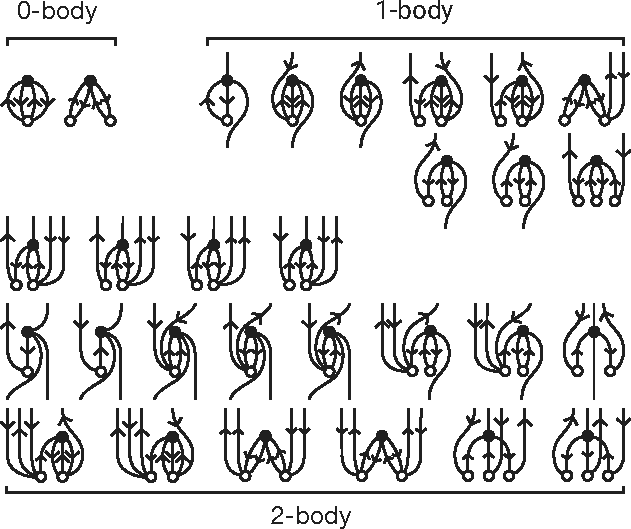
\includegraphics{fig-diagrams-ccsd}
\caption{Diagrammatic representation of $\bar{H}$ of \eqref{eq:cc_heff1}, where open circles represent the excitation cluster operators $\hat{T}_{1}$ and $\hat{T}_{2}$, and filled circles represent the two-body interaction $\hat{H}^{[2]}$.  The diagrams are implicitly antisymmetrized (Hugenholtz diagrams).  Lines connected to $\hat{T}$ are always directed upward because they represent an excitation operator while the directions of external lines connected to $\hat{H}^{[2]}$ are unconstrained.}
\label{fig:diagrams-ccsd}
\end{figure}

The unknown cluster amplitudes in CCSD, $t_{a, i}^{[1]}$ and $t_{a, b, i, j}^{[2]}$, are calculated by left-multiplying \eqref{eq:cc_schrodeq} by $\bra{\Phi}\normord{ \hat a_{i}^\dagger \hat a_{a}}e^{-\hat{T}}$ and $\bra{\Phi}\normord{ \hat a_{i}^\dagger \hat a_{j}^\dagger \hat a_{b} \hat a_{a}}e^{-\hat{T}}$, respectively.
\begin{gather}\label{eq:ccsd1}
\bra{\Phi}\normord{ \hat a_{i}^\dagger \hat a_{a}}\bar{H}_{\mathrm{CC}}\ket{\Phi} = 0 \\
\bra{\Phi}\normord{ \hat a_{i}^\dagger \hat a_{j}^\dagger \hat a_{b} \hat a_{a}}\bar{H}_{\mathrm{CC}}\ket{\Phi} = 0 \notag
\end{gather}
After the Fock matrix has been diagonalized, the diagonal components of \eqref{eq:ccsd1} can be separated and, after expanding the exponent in \eqref{eq:cc_heff1}, the non-vanishing terms of the CCSD amplitude equations become,
\begin{gather}\label{eq:ccsd2}
\bra{\Phi}\normord{ \hat a_{i}^\dagger \hat a_{a}} \hat{H}^{[2]}( \hat{T}_{1} + \hat{T}_{2} + \hat{T}_{1}\hat{T}_{2} + \frac{1}{2}\hat{T}_{1}^{2} + \frac{1}{3!}\hat{T}_{1}^{3} )_{c} \ket{\Phi} = (H_{i,i}^{[1]} - H_{a,a}^{[1]})t_{a, i}^{[1]} \\
\bra{\Phi}\normord{ \hat a_{i}^\dagger \hat a_{j}^\dagger \hat a_{b} \hat a_{a}} \hat{H}^{[2]}( 1 + \hat{T}_{1} + \hat{T}_{2} + \frac{1}{2}\hat{T}_{1}^{2} + \hat{T}_{1}\hat{T}_{2} + \frac{1}{2}\hat{T}_{2}^{2} + \frac{1}{3!}\hat{T}_{1}^{3} + \frac{1}{2}\hat{T}_{1}^{2}\hat{T}_{2} + \frac{1}{4!}\hat{T}_{1}^{4} )_{c} \ket{\Phi} \notag \\
\hspace{10cm} = (H_{i,i}^{[1]} + H_{j,j}^{[1]} - H_{a,a}^{[1]} - H_{b,b}^{[1]})t_{a, b, i, j}^{[2]} \notag
\end{gather}
These non-linear equations are solved using an iterative procedure that begins with an initial guess for the cluster amplitudes which are used to calculate the left-hand side of \eqref{eq:ccsd2}. Dividing by the denominator on the right-hand side gives updated amplitudes which are used to reevaluate the left-hand side. This process is repeated until the amplitudes reach a fixed point. Like the Hartree-Fock iterative procedure, employing similar convergence acceleration techniques can help improve the coupled cluster iterations.

\subsection{Quasigenerate perturbation theory}
\label{subsec:selfenergy}

IM-SRG, in the approach described, provides a means to calculate the ground state energy of any system that is reasonably approximated by a single Slater determinant.  This works well for closed-shell systems, but it does not provide a direct means to obtain the ground state energy of open-shell systems.  While there exist more complicated multi-reference approaches to IM-SRG that can tackle the general problem \cite{Hergert2016165}, we opted to use a perturbative approach, which is simple, inexpensive, and as we shall see in the results, quite effective for many problems.

Quasidegenerate perturbation theory (QDPT) is an extension to the traditional perturbation theory framework that incorporates multiple reference states.   It provides us with a simple means to extract ground state energies of open-shell systems that are only a few particles away from a closed-shell system.  In particular, it allows us to calculate \textit{addition energies} $\varepsilon_a$ and \textit{removal energies} $\varepsilon_i$ of such systems, which we define as:
\begin{align}
  \varepsilon_a &\equiv E_{\Phi_a} - E_{\Phi} \\
  \varepsilon_i &\equiv E_{\Phi} - E_{\Phi_i}
\end{align}
where the meaning of $\Phi_p$ is defined in \eqref{eq:quasisd}, $i$ is restricted to labels of occupied states, and $a$ is restricted to labels of unoccupied states.

In QDPT, solutions of an approximate one-body Hamiltonian $\hat{H}^{[1]}$ form the basis of the model space.  One begins by assuming the existence of an operator $\hat{\Omega}$, known as the \textit{wave operator}, that maps some set of states $\tilde \Psi^{\mathrm{o}}_u$ within the model space to the exact ground state $\Psi_u$:
\begin{align} \label{eq:omega-condition1}
  \Psi_u = \hat \Omega \tilde \Psi^{\mathrm{o}}_u
\end{align}
The states $\tilde \Psi^{\mathrm{o}}_u$ consist of some mixture of the eigenstates $\Psi^{\mathrm{o}}_{u'}$ of the approximate Hamiltonian $\hat{H}^{[1]}$.

There is some freedom in the choice of the wave operator $\hat \Omega$.  We assume it has the following form:
\begin{align} \label{eq:omega-condition2}
  \hat \Omega = \hat P + \hat Q \hat \Omega \hat P
\end{align}
where $\hat P$ projects any state into the model space and $\hat Q$ is the complement of $\hat P$.  This entails that the exact states $\Psi_u$ is no longer normalized but instead satisfies the so-called intermediate normalization: $\langle \Psi_u | \tilde \Psi^{\mathrm{o}}_u \rangle = 1$.

Making use of the assumptions in  \eqref{eq:omega-condition1} and \eqref{eq:omega-condition2}, one can derive from the Schr\"odinger equation the generalized Bloch equation, the principal equation of QDPT:
\begin{gather*}
  [\hat \Omega, \hat{H}^{[1]}] =
  (1 - \hat \Omega) \hat V \Omega
\end{gather*}
where $\hat V \equiv \hat H - \hat{H}^{[1]}$ is the perturbation.  The
commutator on the left may be ``inverted'' using the resolvent approach
(\cite{shavitt2009many}, p.\ 50), resulting in:
\begin{align*}
  \hat Q \Omega \hat P_u =
  \hat R_u (1 - \hat \Omega) \hat V \Omega \hat P_u
\end{align*}
where $\hat R_u \equiv \hat Q (E_u - \hat Q \hat{H}^{[1]} \hat Q)^{-1} \hat Q$ defines the resolvent and $\hat P_u$ is the projection operator that projects any state onto $\Psi^{\mathrm{o}}_u$.  As is standard in perturbation theory, we now assume $\hat \Omega$ can be expanded as a series of terms of increasing order, as quantified by the power of the perturbation $\hat V$:
\begin{align*}
  \hat \Omega = \hat P +
  \hat Q\bigl(\hat \Omega^{(1)} + \hat \Omega^{(2)} + \cdots\bigr) \hat P
\end{align*}
This leads to a recursion relation of $\hat \Omega$ that enables $\hat \Omega$ to be calculated up to any order, as least in principle.  Up to third order, we have:
\begin{align*}
  &\hat \Omega^{(1)} \hat P_u = \hat R_u \hat V \hat P_u \\
  &\hat \Omega^{(2)} \hat P_u =
    \hat R_u \biggl(
    \hat V \hat R_u
    - \sum_v \hat R_v \hat V \hat P_v
    \biggr) \hat V \hat P_u \\
  &\hat \Omega^{(3)} \hat P_u =
    \hat R_u \biggl(
    \hat V \hat R_u \hat V \hat R_u
    - \hat V \hat R_u \sum_v \hat R_v \hat V \hat P_v \\
  &\qquad\qquad
    - \sum_v \hat R_v \hat V \hat P_v \hat V \hat R_u
    - \sum_v \hat R_v \hat V \hat R_v \hat V \hat P_v \\
  &\qquad\qquad
    + \sum_v \hat R_v \sum_w \hat R_w \hat V \hat P_w \hat V \hat P_v
    \biggr) \hat V \hat P_u
\end{align*}

\begin{figure}
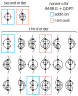
\includegraphics{fig-diagrams-sfe}
\caption{Diagrammatic form of the second- and third-order QDPT corrections.  The diagrams are implicitly antisymmetrized (Hugenholtz diagrams), but also have implicit denominators as with many-body perturbation theory.  When QDPT is performed on IM-SRG-evolved Hamiltonians, many of the diagrams vanish.  The remaining nonvanishing diagrams for addition energy are highlighted in blue and for removal energy are highlighted in red.}
\label{fig:diagrams-sfe}
\end{figure}

To make the equations more concrete, we further assume that each reference state $\ket{\Psi^{\mathrm{o}}_u} \equiv \ket{\Phi_u}$, i.e.\ each reference state is simply a Slater determinant constructed by adding or removing a single particle $u$ to a closed-shell reference state $\Phi$, which itself may have been obtained earlier from HF and/or IM-SRG.  Thus, the number of reference states for QDPT is equal to the number of particles in either the lowest unfilled shell or the highest filled shell of $\ket{\Phi}$, depending on whether we are considering addition or removal energies.

We can then express the perturbation expansion in terms of summations over matrix elements as we had done before for the IM-SRG flow equation, again with the aid of Wick's theorem or diagrammatic techniques.  This leads to the following expression for the second-order correction:
\begin{align*}
  \varepsilon_p^{(2)}
  &=
    \sum_{i, a, b} \frac{n_i \bar{n}_a \bar{n}_b |H^{[2]}_{p, i, a, b}|^2}{2 \Delta_{\{p, i\}, \{a, b\}}}
    - \sum_{i, j, a} \frac{n_i n_j \bar{n}_a |H^{[2]}_{i, j, p, a}|^2}{2 \Delta_{\{i, j\}, \{p, a\}}}
\end{align*}
where the M\o ller--Plesset denominators $\Delta$ are defined in \eqref{eq:moellerplessetdenominator}.  The above expression is depicted in Figure \ref{fig:diagrams-sfe}.  Since there are numerous terms in the third-order correction $\varepsilon_p^{(3)}$, they are listed in diagrammatic form in Figure \ref{fig:diagrams-sfe}.  We will refer to QDPT to third order as ``QDPT3''.

Taking into account the perturbation corrections, one can extract reasonably accurate addition and removal energies for single-particle states near the Fermi level via:
\begin{align*}
  \varepsilon_p = H^{[1]}_{p, p} + \varepsilon_p^{(2)} + \varepsilon_p^{(3)}
\end{align*}

There is some degree of synergy between IM-SRG and QDPT: a generator that decouples the ground state energy will necessarily drive certain classes of matrix elements to zero.  This means certain kinds of vertices in the diagrams become forbidden, reducing the number of nonzero diagrams at third order from 18 to only 4.

\subsection{Equations of motion methods}

Particle attached and particle removed equations of motion (EOM) methods can be coupled with either IM-SRG or coupled cluster calculations. The principal idea is that one may construct a ladder operator $\hat{X}$ that promotes the $N$-particle ground state to any state in the $N + 1$ or $N - 1$ spectrum,
\begin{equation}\label{eq:ladder_def}
  \ket{\Psi^{(N \pm 1)}_u}  = \hat{X}^{(N \pm 1)}_u \ket{\Psi^{(N)}_0},
\end{equation}
where $\hat{X}$ is in principle a linear combination of excitation and de-excitation operators that change particle number by one,
\begin{align}
  \label{eq:gen_attached}
  \hat{X}^{(N+1)}_u &= \sum_p \bar{n}_p x^{[1,0]}_p  \hat{a}^\dagger_p + \frac{1}{2} \sum^{[2,1]}_{p, q, r} \bar{n}_p \bar{n}_q n_r x_{p, q, r} \hat{a}^\dagger_p \hat{a}^\dagger_q \hat{a}_r + \cdots,  \\
  \label{eq:gen_removed}
  \hat{X}^{(N-1)}_u &= \sum_p n_p x_p^{[0,1]} \hat{a}_p + \frac{1}{2} \sum_{p, q, r} n_p n_q \bar{n}_r  x^{[1,2]}_{p, q, r} \hat{a}^\dagger_r \hat{a}_q \hat{a}_p  + \cdots.
\end{align}
Substitution of \eqref{eq:ladder_def} into the energy eigenvalue problem
\begin{gather*}
  \hat H \ket{\Psi_u^{(N \pm 1)}} = E^{(N\pm1)}_u \ket{\Psi_u^{(N \pm 1)}}
\end{gather*}
gives
\begin{equation}\label{eq:EOM}
  [\hat{H}, \hat{X}^{(N \pm 1)}_u] \ket{\Psi^{(N)}_0} = \pm \varepsilon^{(\pm)}_u \hat{X}^{(N \pm 1)}_u \ket{\Psi^{(N)}_0},
\end{equation}
which constitutes a generalized eigenvalue problem for the amplitudes $x$, where $\varepsilon^{(\pm)}_u$ are the single-particle addition ($+$) and removal ($-$) energies. The quality of this calculation depends on the ansatz for the $N$-particle ground state, as well as the systematically improvable truncation on the ladder operators. In this work we include 1p and 2p1h excitations in the $N + 1$ ladder operator and likewise 1h and 2h1p operators for the $N - 1$ ladder operators.

\subsubsection*{EOM-IM-SRG}
After a single-reference ground state IM-SRG calculation, the Hamiltonian has been rotated such that the reference state is an eigenfunction with corresponding eigenvalue $E^{(N)}_0$, which is the correlated $N$-particle ground state energy. The EOM equation is therefore
\begin{equation}\label{eq:EOMIMSRG}
  [\bar{H},\bar{X}^{(N \pm 1)}_u] \ket{\Phi^{(N)}_0} = \pm \varepsilon^{(\pm)}_u \bar{X}^{(N \pm 1)}_u \ket{\Phi^{(N)}_0},
\end{equation}
where bars denote rotated operators. Now the reference state is used in place of the bare correlated ground state. The ground state IM-SRG procedure has implicitly re-summed contributions from higher order excitations (3-particle-2-hole, 2-particle-3-hole, 2-particle-3-hole, 4-particle-3-hole, \ldots) into the lower order amplitudes of the ladder operators (1-particle-0-hole, 0-particle-1-hole, 2-particle-1-hole, 1-particle-2-hole).

Despite these gains, the EOM calculation is still a partial diagonalization method, limited by the truncation to 2-particle-1-hole and 1-particle-2-hole operators. We expect $N + 1$ (or $N - 1$) states to be described appropriately by EOM-IM-SRG if their wavefunctions are dominated by 1-particle-0-hole (or 0-particle-1-hole) contributions in the rotated frame. We use partial norms of the EOM ladder operators to make this determination:
\begin{align}
  \label{eq:partial_norms_p}
  n_{\text{1-particle}} &= \sqrt{\sum_p \bar{n}_p | \bar{x}^{[1,0]}_p |^2},\\
  \label{eq:partial_norms_h}
  n_{\text{1-hole}} &= \sqrt{\sum_p n_p | \bar{x}^{[0,1]}_p |^2}.
\end{align}
Large single particle partial norms indicate that the EOM truncation is valid for the relevant state. States with lower single particle norms should be treated by with a higher EOM approximation, which can be accomplished directly or perturbatively \cite{PhysRevC.95.044304}.

\subsubsection*{EOM-CC}
\label{subsec:eomcc}
Like EOM-IM-SRG, the equation-of-motion technique can be applied after a coupled-cluster ground-state calculation, by using the coupled-cluster effective Hamiltonian.  Here, the non-Hermitian nature of $\bar{H}_{\mathrm{CC}}$ becomes apparent.  In this case, in addition to constructing excitation ladder operators \eqref{eq:gen_attached} and \eqref{eq:gen_removed} that correspond to the right-eigenvectors of the generalized eigenvalue problem \eqref{eq:EOMIMSRG}, there exist analogous de-excitation ladder operators, $\hat{L}^{(N+1)}$ and $\hat{L}^{(N-1)}$, that correspond to the left-eigenvectors,
\begin{align}
  \label{eq:left_attached}
    \hat{L}^{(N+1)}_w &= \sum_p \bar{n}_p l^{[1,0]}_p  \hat{a}_p + \frac{1}{2} \sum_{p, q, r} \bar{n}_p \bar{n}_q n_r l^{[2,1]}_{p, q, r} \hat{a}^\dagger_r \hat{a}_q \hat{a}_p + \cdots,  \\
  \label{eq:left_removed}
    \hat{L}^{(N-1)}_w &= \sum_p n_p l_p^{[0,1]} \hat{a}^\dagger_p + \frac{1}{2} \sum_{p, q, r} n_p n_q \bar{n}_r  l^{[1,2]}_{p, q, r} \hat{a}^\dagger_p  \hat{a}^\dagger_q \hat{a}_r + \cdots.
\end{align}
These left-eigenvectors satisfy the left-eigenvalue problem, with left-eigenvalues $\varepsilon^{(\pm)}_w$, analogous to \eqref{eq:EOMIMSRG},
\begin{equation}\label{eq:left_EOM}
  \bra{\Phi^{(N)}_0} [\bar{H},\bar{L}^{(N \pm 1)}_w] = \pm \varepsilon^{(\pm)}_w \bra{\Phi^{(N)}_0} \bar{L}^{(N \pm 1)}_w,
\end{equation}
and form a bi-orthogonal set with the right-eigenvectors, $\braket{\bar{L}^{(N \pm 1)}_w}{\bar{X}^{(N \pm 1)}_u} = \delta_{w,u}$.

In this paper, because the interaction is real and thus the effective Hamiltonian is real, the left- and right-eigenvalues are equivalent. In addition, while the the left- and right-eigenvectors are generally not equal, the differences in their single-particle \eqref{eq:partial_norms_p} or single-hole \eqref{eq:partial_norms_h} natures are, in practice, not significant.  Therefore, only the right-eigenvectors are used in this paper.

\section{Results}
\label{sec:results}

\subsection{Methodology}
\label{subsec:methodology}

\begin{figure}
  \centering
  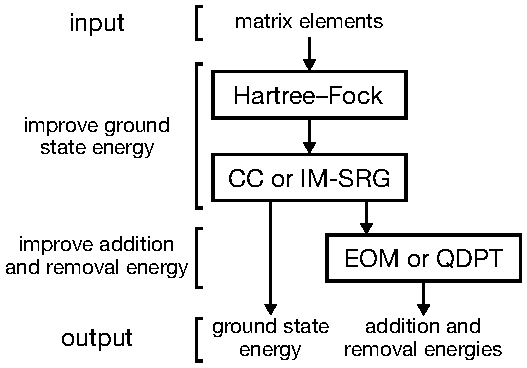
\includegraphics{figures/fig-methods}
  \caption{A schematic view of the various ways in which many-body methods in this paper could be combined to calculate ground state, addition, and removal energies.}
  \label{fig:methods}
\end{figure}

There is great amount of flexibility in the application of many-body methods.  The approaches we use is depicted in Figure \ref{fig:methods}.  Such an ordering maximizes the benefits of each method: Hartree--Fock acts as an initial, crude procedure to ``soften'' the Hamiltonian, followed by IM-SRG or CC to refine the ground state energy, and then finally QDPT or EOM to refine the addition and removal energies.

The general process begins with the input matrix elements \eqref{eq:interactionintegral}, computed exactly using the \texttt{OpenFCI} software library \cite{2008arXiv0810.2644K}.  Internally, \texttt{OpenFCI} calculates the interaction integrals in the center-of-mass frame using Gauss--Hermite quadrature and transforms them back into the laboratory frame to produce matrix elements suitable for use in our many-body methods.

Afterward, there are several paths through which one can traverse Figure \ref{fig:methods} to obtain output observables.  We shall primarily focus on the three combinations: (a) HF + IM-SRG(2) + QDPT3, (b) HF + IM-SRG(2) + EOM2, and (c) HF + CCSD + EOM2.

It is possible to omit some steps of the process.  For example, one can omit HF, but continue with the remaining two steps.  While this is doable, from our experience Hartree--Fock significantly improves the results of the later post-HF methods at very low cost compared to the post-HF methods.  Therefore, in practice there is little reason to omit HF.  We will however investigate the effects of removing one or more of the post-HF methods.

Since every calculation in this paper is begins with the Hartree--Fock stage, we will not explicitly state ``HF'' unless there is no post-HF method used at all, in which case we write ``HF only''.

All calculations of ground state energy $E_N$ in this paper are restricted to cases where the number of particles $N$ is a magic number, i.e.\ a \textit{closed shell} system (see Figure \ref{fig:shell-structure} for an illustration of the shell structure).  This is a limitation of the many-body methods used in this paper and while there are ways to overcome this limit they are beyond the scope of this paper (see Section \ref{sec:conclusions} for some ideas).  Addition/removal energies $\varepsilon^{(\pm)}$ are similarly restricted in that we only calculate the energy difference between $E_N$ of a closed shell system and $E_{N \pm 1}$ of the same system but with one particle added/removed:
\begin{align*}
  \varepsilon^{(+)} &\equiv E_{N + 1} - E_N \\
  \varepsilon^{(-)} &\equiv E_N - E_{N - 1}
\end{align*}

Ideally, ground state energy should be characterized entirely by the two system parameters $(N, \omega)$, where $N$ is number of particles and $\omega$ is the oscillator frequency.  However, the methods that we study are limited to a \emph{finite} (truncated) basis and therefore their results are dependent on the level of truncation.  This is characterized by $K$, the total number of shells in the single-particle basis.  Thus, results are generally presented as a graph plotted against $K$.  In Section \ref{subsec:extrapolation} discuss how to estimate results as $K \to \infty$ (infinite-basis limit) through \textit{extrapolations}.

The addition and removal energies are similar, but they require an additional parameter: the total orbital angular momentum $M_\ell$, defined as the sum of the $m_\ell$ of each particle.  This is due to the presence of multiple states with near-degenerate energies.  For this paper, we will consider exclusively the addition/removal energies with the lowest $|M_\ell|$ subject to the constraint that the particle added/removed lies within the next/last shell.  This means the $N + 1$ states of interest are those with $|M_\ell| = K_{\mathrm{F}} \bmod 2$ where $K_{\mathrm{F}}$ is the number of occupied shells, while the $N - 1$ states of interest are those with $|M_\ell| = 1 - (K_{\mathrm{F}} \bmod 2)$.

Not all cases are solvable with our selection many-body methods.  Low frequency systems are particularly strenuous for these many-body methods due to their strong correlations, leading to equations that are difficult and expensive to solve numerically.  Cases where IM-SRG converged too slowly to be feasible or diverged are marked ``n.c.(I)''.  For the extrapolations in Section \ref{subsec:extrapolation}, some fits could not be done due to missing data caused by IM-SRG(2) or CCSD nonconvergence (``n.c.''); others converged but resulted in unphysical $\beta \le 0$ (``n.f.'').  Cases where results are simply unavailable for technical or logistic reasons are left blank in the tables.

Numerical calculations in this paper are performed with a relative precision of about $10^{-5}$ or lower.  This does not necessarily mean the results are as precise as $10^{-5}$, since numerical errors tend to accumulate over the multiple steps of the calculation, thus the precision of the final results is expected to be roughly $10^{-4}$.

\subsection{Comparison between methods}

\subsubsection{Ground state energy}

\begin{table}
  \centering
  \caption{Ground state energy of quantum dots with $N$ particles and an oscillator frequency of $\omega$.  For every row, the calculations performed in a harmonic oscillator basis size with $K$ shells.}
  \label{tab:ground}
  
        \begin{tabular}{S[table-format=2.0]SS[table-format=2.0]S[table-format=3.5]S[table-format=3.5]S[table-format=3.5]S[table-format=3.5]}%
        \toprule
        {$N$} & {$\omega$} & {$K$} & {HF} & {MP2} & {IM-SRG(2)} & {CCSD} \\
        \midrule
6 & 0.1 & 12 & 3.8524 & 3.5516 & 3.4944 & 3.5835 \\
6 & 0.28 & 12 & 8.0196 & 7.6172 & 7.5743 & 7.6360 \\
6 & 1.0 & 12 & 20.7192 & 20.2064 & 20.1742 & 20.2063 \\
\midrule
12 & 0.1 & 15 & 12.9247 & 12.2531 & 12.2212 & 12.3589 \\
12 & 0.28 & 15 & 26.5500 & 25.6524 & 25.6277 & 25.7368 \\
12 & 1.0 & 15 & 66.9113 & 65.7752 & 65.7544 & 65.8166 \\
\midrule
20 & 0.1 & 15 & 31.1686 & 30.0032 & 29.9546 & 30.1745 \\
20 & 0.28 & 15 & 63.5390 & 61.9865 & 61.9645 & 62.1383 \\
20 & 1.0 & 15 & 158.0043 & 156.0533 & 156.0424 & 156.1433 \\
\midrule
30 & 0.1 & 15 & 62.7783 & 61.0766 & 60.8855 & 61.2321 \\
30 & 0.28 & 15 & 126.5597 & 124.2173 & 124.1533 & 124.4149 \\
30 & 1.0 & 15 & 311.8604 & 308.9235 & 308.9306 & 309.0766 \\
\midrule
42 & 0.1 & 20 & 110.7797 & 108.1350 & 108.0604 & 108.5150 \\
42 & 0.28 & 20 & 223.5045 & 219.9270 & 220.0227 & 220.3683 \\
42 & 1.0 & 20 & 547.6832 & 543.2139 & 543.3399 & 543.5423 \\
\midrule
56 & 0.1 & 20 &  &  & {n.c.} & 179.6938 \\
56 & 0.28 & 20 & 363.8784 & 359.1916 & 359.1997 & 359.6744 \\
56 & 1.0 & 20 & 885.8539 & 879.9325 & 880.1163 & 880.3781 \\
\bottomrule\end{tabular}
\end{table}

\begin{figure}
  \centering
  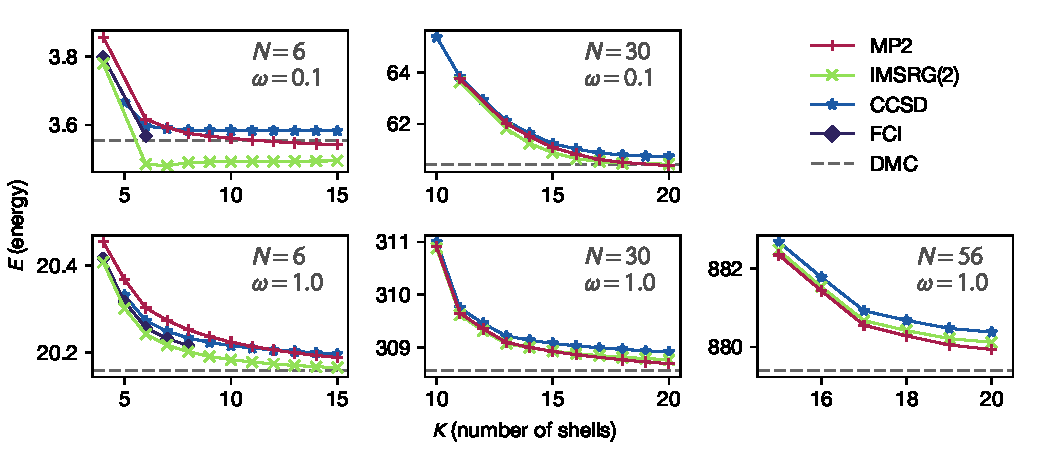
\includegraphics{fig-gs2}
  \caption{Plots of ground state energy of quantum dots with $N$ particles and an oscillatory frequency of $\omega$ against the number of shells $K$.  Since DMC does not utilize a finite basis, the horizontal axis is irrelevant and DMC results are plotted as horizontal lines.}
  \label{fig:gs}
\end{figure}

In Figure \ref{fig:gs} we display a selection of ground state energies calculated using HF + IM-SRG(2) and HF + CCSD as described in Section \ref{subsec:methodology}.  We also include results from M\o ller--Plesset perturbation theory to second order (MP2), DMC \cite{hoegberget2013thesis}, and FCI \cite{olsen2013thesis} for comparison where available.

We do not include results from ``HF only'' to avoid overshadowing the comparatively smaller differences between the non-HF results in the plots.  Some HF results can be found Figure \ref{fig:by-freq-10-6-normal} instead.  Generally, HF ground state energies differ from the non-HF ones by a few to several percent, whereas non-HF energies tend to differ from each other by less than a percent.

With respect to the number of shells, both IM-SRG(2) and CCSD appear to converge slightly faster than second order perturbation theory (MP2), likely due to the presence of higher order corrections in IM-SRG(2) and CCSD.

There are a few cases where the IM-SRG over-corrects the result, leading to an energy lower than the quasi-exact DMC results.  This is not unexpected given that, unlike Hartree--Fock, IM-SRG is non-variational in the presence of operator truncations, which cause small unitarity violations.  This over-correction tends to occur when the frequency is low (high correlation), or somewhat counterintuitvely, when \emph{few} particles are involved.

\subsubsection{Addition and removal energies}

\begin{table}
  \centering
  \caption{Addition energy of quantum dot systems.  See Table \ref{tab:ground} for details.}
  \label{tab:add}
  
        \begin{tabular}{SSSSSSS}%
        \toprule
        {$N$} & {$\omega$} & {$K$} & {HF} & {IM-SRG(2)} & {IMSRG(2)} & {CCSD} \\
        {} & {} & {} & {+QDPT3} & {+QDPT3} & {+EOM} & {+EOM} \\
        \midrule
6 & 0.1 & 15 & 1.2286 & 1.2023 &  & 1.1860 \\
6 & 0.28 & 15 & 2.5216 & 2.5008 & 2.4915 & 2.4831 \\
6 & 1.0 & 15 & 6.4803 & 6.4544 & 6.4529 & 6.4447 \\
\midrule
12 & 0.1 & 15 & 1.9701 & 1.9233 &  & 1.9015 \\
12 & 0.28 & 15 & 3.9893 & 3.9389 & 3.9357 & 3.9208 \\
12 & 1.0 & 15 & 9.9745 & 9.9261 & 9.9282 & 9.9146 \\
\midrule
20 & 0.1 & 15 & 2.8037 & 2.7186 &  & 2.7122 \\
20 & 0.28 & 15 & 5.6189 & 5.5397 & 5.5416 & 5.5234 \\
20 & 1.0 & 15 & 13.8476 & 13.7810 & 13.7858 & 13.7683 \\
\midrule
30 & 0.1 & 15 & 3.8326 & 3.6929 &  & 3.6905 \\
30 & 0.28 & 15 & 7.4321 & 7.2970 & 7.3117 & 7.2916 \\
30 & 1.0 & 15 & 17.9969 & 17.9046 & 17.9117 & 17.8904 \\
\midrule
42 & 0.1 & 15 &  &  &  & 4.8996 \\
42 & 0.28 & 15 & 9.5480 & 9.3795 &  & 9.3576 \\
42 & 1.0 & 15 & 22.4649 & 22.3454 & 22.3547 & 22.3291 \\
\midrule
56 & 0.1 & 20 &  &  &  & 5.7661 \\
56 & 0.28 & 20 & 11.3932 & 11.1683 &  & 11.1518 \\
56 & 1.0 & 20 & 27.0513 & 26.9033 &  & 26.8842 \\
\bottomrule\end{tabular}
\end{table}

\begin{table}
  \centering
  \caption{Removal energy of quantum dot systems.  See Table \ref{tab:add} for details.}
  \label{tab:rm}
  
        \begin{tabular}{S[table-format=2.0]SS[table-format=2.0]S[table-format=3.5]S[table-format=3.5]S[table-format=3.5]S[table-format=3.5]}%
        \toprule
        {$N$} & {$\omega$} & {$K$} & {HF} & {IM-SRG(2)} & {IMSRG(2)} & {CCSD} \\
        {} & {} & {} & {+QDPT3} & {+QDPT3} & {+EOM} & {+EOM} \\
        \midrule
6 & 0.1 & 12 & 1.04565 & 0.94963 & 0.95512 & 1.00553 \\
6 & 0.28 & 12 & 2.11603 & 2.03492 & 2.04014 & 2.07887 \\
6 & 1.0 & 12 & 5.25233 & 5.19702 & 5.19917 & 5.22404 \\
\midrule
12 & 0.1 & 15 & 1.79945 & 1.69594 &  & 1.75038 \\
12 & 0.28 & 15 & 3.62545 & 3.53364 & 3.53688 & 3.57832 \\
12 & 1.0 & 15 & 8.87953 & 8.81147 & 8.81121 & 8.84207 \\
\midrule
20 & 0.1 & 15 & 2.62929 & 2.51506 &  & 2.57377 \\
20 & 0.28 & 15 & 5.26538 & 5.16450 & 5.16661 & 5.21140 \\
20 & 1.0 & 15 & 12.80026 & 12.72194 & 12.72037 & 12.75650 \\
\midrule
30 & 0.1 & 15 & 3.61723 & 3.48885 &  & 3.54381 \\
30 & 0.28 & 15 & 7.04682 & 6.94022 & 6.94090 & 6.99016 \\
30 & 1.0 & 15 & 17.00690 & 16.92781 & 16.92495 & 16.96460 \\
\midrule
42 & 0.1 & 20 & 4.52092 & 4.38676 &  & 4.44511 \\
42 & 0.28 & 20 & 8.88307 & 8.77647 &  & 8.82628 \\
42 & 1.0 & 20 & 21.43339 & 21.34535 &  & 21.38485 \\
\midrule
56 & 0.1 & 20 &  & {n.c.} & {n.c.} & 5.63405 \\
56 & 0.28 & 20 & 10.96015 & 10.84707 &  & 10.89566 \\
56 & 1.0 & 20 & 26.09515 & 26.00937 &  & 26.05068 \\
\bottomrule\end{tabular}
\end{table}

\begin{figure}
  \centering
  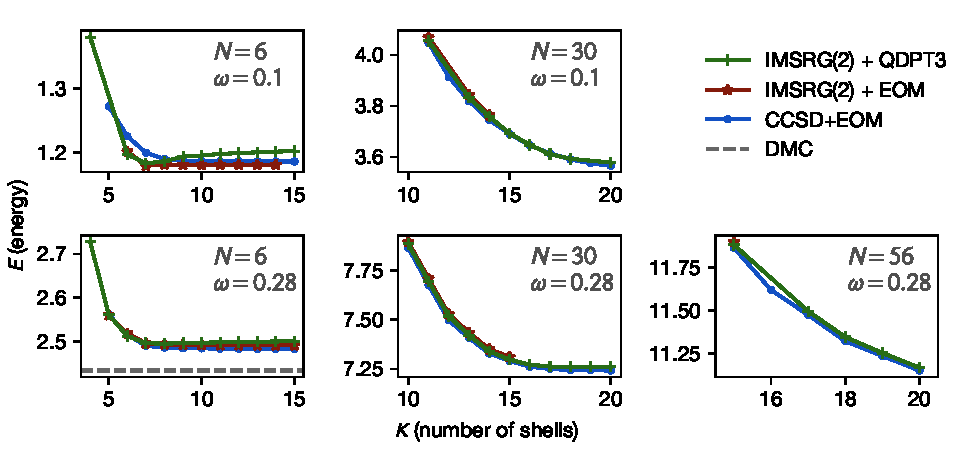
\includegraphics{fig-add2}
  \caption{Addition energies for a selection of quantum dot parameters.  See Figure \ref{fig:gs} for details.}
  \label{fig:add}
\end{figure}

\begin{figure}
  \centering
  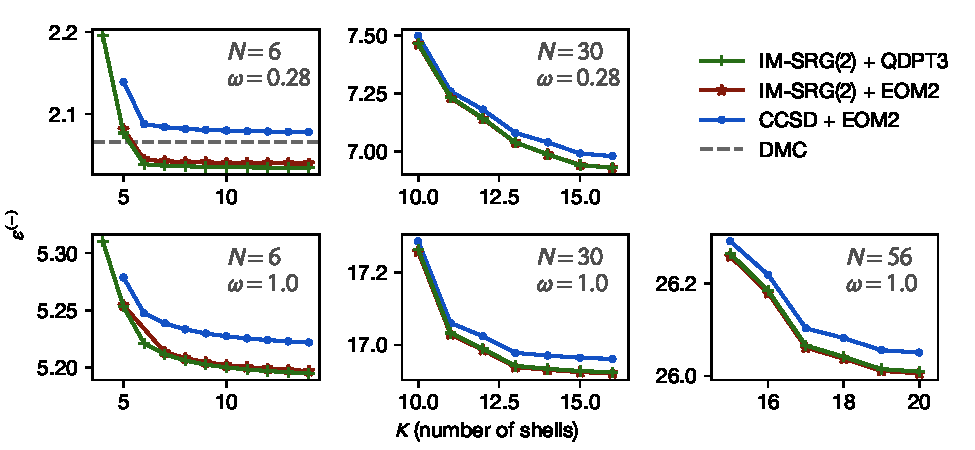
\includegraphics{fig-rm2}
  \caption{Removal energies for a selection of quantum dot parameters.  See Figure \ref{fig:add} for details.}
  \label{fig:rm}
\end{figure}

The results of our addition and removal energy calculations are summarized in Figure \ref{fig:add} and Figure \ref{fig:rm} respectively.  The figures show the the addition/removal energies for using the approaches mentioned in Section \ref{subsec:methodology}.  Where available, results from diffusion Monte Carlo (DMC) \cite{PhysRevB.84.115302} are shown as a dashed line.

As before, we do not include results from ``HF only'' in these plots as they are significantly further from the rest.  Analogously, we also exclude results from pure IM-SRG (i.e.\ without QDPT nor EOM) or pure CCSD, as QDPT or EOM both add significant contributions to addition and removal energies.  Some HF only and pure IM-SRG results can be seen in Figure \ref{fig:by-freq-10-6-normal}.

There is strong agreement between IM-SRG(2) + QDPT3 and IM-SRG(2) + EOM2 in many cases, and slightly weaker agreement between the IM-SRG and CCSD families.  This suggests that the EOM2 corrections are largely accounted for by the inexpensive QDPT3 method.  However, in some cases, most notably with few particles and high correlations (low frequency), the IM-SRG(2) + QDPT3 result differs significantly from both IM-SRG(2) + EOM2 and CCSD + EOM2.

\subsection{Rate of convergence}

\begin{figure}
  \centering
  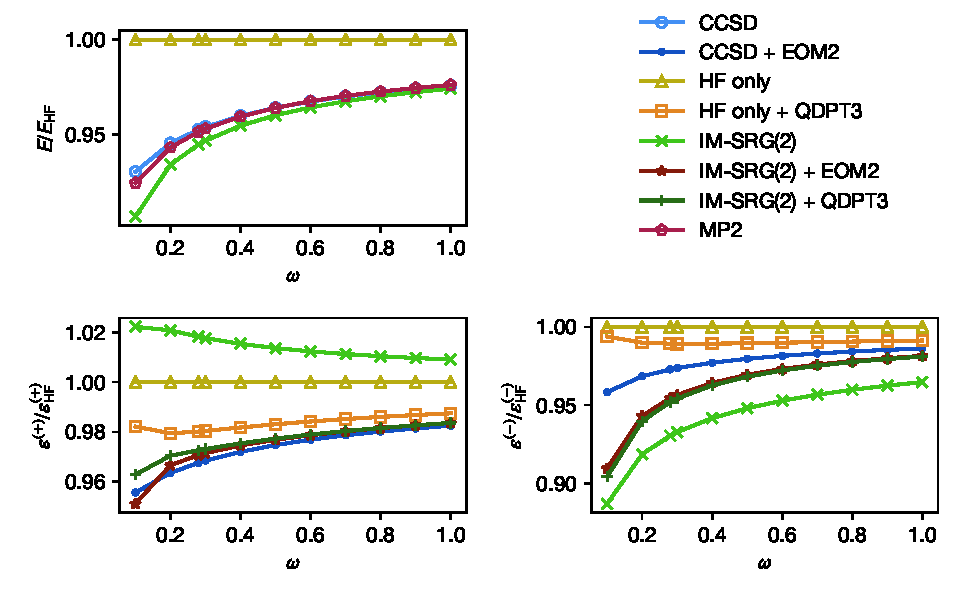
\includegraphics{fig-by-freq-10-6-normal}
  \caption{The behavior of ground state, addition, and removal energies as a function of the oscillator frequency $\omega$, with $K = 10$ shells in the basis.  The energy is normalized with respect to the Hartree--Fock values to magnify the differences.  Lower frequency leads to stronger correlations and thereby a more difficult problem.  The fact that CCSD and MP2 are similar is likely coincidence as they cross at around 12 shells and then diverge again (not shown in this plot).}
  \label{fig:by-freq-10-6-normal}
\end{figure}

\begin{figure}
  \centering
  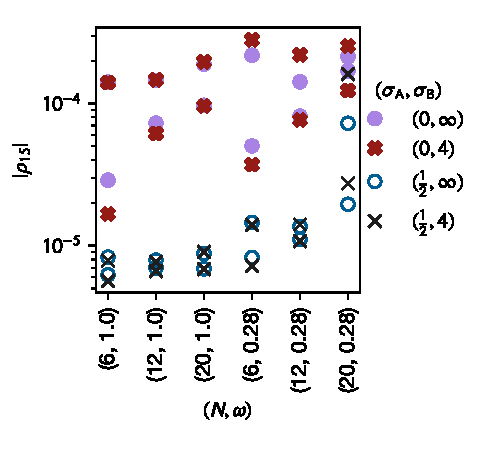
\includegraphics{fig-rel-slopes2}
  \caption{The impact of the interaction on convergence of addition and removal energies using IM-SRG(2) + QDPT3.  For clarity, the plot does not distinguish between addition and removal energies.  The horizontal axis shows the system parameters, where $N$ is the number of particles and $\omega$ is the oscillator frequency.  The vertical axis shows $|\rho_{15}|$ (``relative slope''), which estimates the rate of convergence at 15 total shells.  The lower the value of $|\rho_{15}|$, the faster the convergence.  The data points are categorized by the interactions.  The trends suggest that the singular short-range part of the interaction has a much stronger impact on the convergence than the long-range tail.}
  \label{fig:rel-slopes}
\end{figure}

To analyze the rate of convergence more quantitatively, we shall define $\rho_K$ as the relative backward difference of the energy (\textit{relative slope}):
\begin{align*}
  \rho_K = \frac{\varepsilon_{K} - \varepsilon_{K - 1}}{\varepsilon_K}
\end{align*}
The denominator allows the quantity to be meaningfully compared between different systems.  We expect this quantity to become increasingly small as the calculations converge.

In Figure \ref{fig:rel-slopes}, we plot the $\rho_{15}$ for IM-SRG(2) + QDPT3.  The many-body methods were tested against a \emph{modified} Coulomb-like interaction, parametrized by two lengths $\sigma_{\mathrm{A}}$ and $\sigma_{\mathrm{B}}$ that characterize the range of the interaction:
\begin{align}
  V_{\sigma_{\mathrm{A}}, \sigma_{\mathrm{B}}}(r) \equiv \frac{(1 + c)^{1 - 1/c}}{c} \left(1 - \E^{-r^2 / (2 \sigma_{\mathrm{A}}^2)}\right) \E^{-r^2 / (2 \sigma_{\mathrm{B}}^2)} \frac{1}{r}
\end{align}
where $c \equiv \sqrt{\sigma_{\mathrm{B}} / \sigma_{\mathrm{A}}}$.  The coefficient is chosen to ensure the peak of the envelope remains at unity.  With $(\sigma_{\mathrm{A}}, \sigma_{\mathrm{B}}) = (0, \infty)$ one recovers the original Coulomb interaction.  By increasing $\sigma_{\mathrm{A}}$ one can truncate the short-range part of the interaction, and analogously by increasing $\sigma_{\mathrm{B}}$ one can truncate the long-range part of the interaction.  For our numerical experiments we considered the following four combinations of $(\sigma_{\mathrm{A}}, \sigma_{\mathrm{B}})$: $(0, \infty)$, $(\frac{1}{2}, \infty)$, $(0, 4)$, $(\frac{1}{2}, 4)$.

Reducing short-range part of the interaction appears improves the rate of convergence substantially.  Many of the cases have reached the precision of the ODE solver ($10^{-5}$ to $10^{-6}$).  In contrast, eliminating the long-range part of the interaction had very little effect.  This suggests that the main cause of the slow convergence lies in the highly repulsive, short-ranged part of the interaction, which leads to the presence of nondifferentiable cusps (the so-called \textit{Coulomb cusps}) in the exact wave functions that are difficult to reproduce exactly using linear combinations of the smooth harmonic oscillator wave functions.

The convergence is negatively impacted at lower frequencies and, to a lesser extent, by the increased number of particles.  Both are expected: lower frequencies increase the correlation in the system, while higher number of particles naturally require more shells to converge.

In general, there does not appear to be any difference between the convergence behavior of addition energies as compared to that of removal energies.

\subsection{Extrapolation}
\label{subsec:extrapolation}

\begin{table}
  \centering
  \caption{Extrapolated ground state energies for quantum dots with fit uncertainties.  The uncertainties are computed from the approximate Hessian constructed by Levenberg-Marquardt fitting algorithm.  Extrapolations are done using 5-point fits where the number of shells $K$ ranges between $K_{\text{stop}} - 4$ and $K_{\text{stop}}$ (inclusive).}
  \label{tab:ground-extrapolated}
  
        \begin{tabular}{S[table-format=2.0]SS[table-format=2.0]S[table-format=4.6]S[table-format=4.6]S[table-format=4.6]}%
        \toprule
        {$N$} & {$\omega$} & {$K_{\text{stop}}$} & {MP2} & {IM-SRG(2)} & {CCSD} \\
        \midrule
6 & 0.1 & 14 & 3.5108(4) & 3.4963(5) & 3.58183(2) \\
6 & 0.28 & 14 & 7.5608(3) & 7.56971(2) & 7.62812(7) \\
6 & 1.0 & 14 & 20.12998(5) & 20.1481(3) & 20.1791(3) \\
\midrule
12 & 0.1 & 16 & 12.198(7) & 12.2217(2) & 12.3575(4) \\
12 & 0.28 & 16 & 25.548(1) & 25.6146(1) & 25.7190(2) \\
12 & 1.0 & 16 & 65.627(2) & 65.6970(7) & 65.7579(8) \\
\midrule
20 & 0.1 & 16 & 29.87(5) & 29.950(1) & 30.13(2) \\
20 & 0.28 & 16 & 61.88(1) & 61.946(3) & 62.114(5) \\
20 & 1.0 & 16 & 155.758(3) & 155.912(4) & 156.010(3) \\
\midrule
30 & 0.1 & 16 & 59.8(2) & {n.c.} & 60.3(2) \\
30 & 0.28 & 16 & 123.95(8) & 124.00(4) & 124.26(5) \\
30 & 1.0 & 16 & 308.80(5) & 308.85(3) & 309.00(3) \\
\midrule
42 & 0.1 & 20 & 106.3(4) & 107.0(1) & 107.1(4) \\
42 & 0.28 & 20 & 219.6(2) & 219.89(8) & 220.2(1) \\
42 & 1.0 & 20 & 542.686(9) & 543.074(3) & 543.276(4) \\
\midrule
56 & 0.1 & 20 & 172.9(6) & {n.c.} & {n.c.} \\
56 & 0.28 & 20 & 357.3(6) & {n.c.} & 358.1(5) \\
56 & 1.0 & 20 & 879.86(8) & 880.07(7) & 880.33(7) \\
\bottomrule\end{tabular}
\end{table}

\begin{table}
  \centering
  \caption{Extrapolated addition energies for quantum dots with fit uncertainties.  See Table \ref{tab:ground-extrapolated} for details.}
  \label{tab:add-extrapolated}
  
        \begin{tabular}{S[table-format=2.0]SS[table-format=2.0]S[table-format=3.6]S[table-format=3.6]S[table-format=3.6]}%
        \toprule
        {$N$} & {$\omega$} & {$K_{\text{stop}}$} & {IM-SRG(2)} & {IMSRG(2)} & {CCSD} \\
        {} & {} & {} & {+QDPT3} & {+EOM} & {+EOM} \\
        \midrule
6 & 0.1 & 14 & 1.206(2) & 1.18095(5) & 1.18581(2) \\
6 & 0.28 & 14 & 2.63(8) & 2.49039(2) & 2.48213(4) \\
6 & 1.0 & 14 & 6.4536(1) & 6.4491(7) & 6.440747(1) \\
\midrule
12 & 0.1 & 16 & {{n.f.}} & 1.909274(1) & 1.90139(2) \\
12 & 0.28 & 16 & 3.925(5) & 3.9339(3) & 3.918521(9) \\
12 & 1.0 & 16 & 9.9235(2) & 9.9235(5) & 9.9070(1) \\
\midrule
20 & 0.1 & 16 & 2.708(4) &  & 2.682(2) \\
20 & 0.28 & 16 & 5.53915(1) &  & 5.52180(7) \\
20 & 1.0 & 16 & 13.7759(8) &  & 13.760(2) \\
\midrule
30 & 0.1 & 16 & {n.c.} & {n.c.} & 3.40(2) \\
30 & 0.28 & 16 & 7.18(3) & 7.18(5) & 7.16(4) \\
30 & 1.0 & 16 & 17.897(4) & 17.902(6) & 17.880(6) \\
\midrule
42 & 0.1 & 20 & 4.19(6) &  & 4.33(2) \\
42 & 0.28 & 20 & 9.068(6) &  & 9.05(1) \\
42 & 1.0 & 20 & 22.2943(7) &  & 22.2768(9) \\
\midrule
56 & 0.1 & 20 & {n.c.} & {n.c.} & {n.c.} \\
56 & 0.28 & 20 & {n.c.} & {n.c.} & 10.7(3) \\
56 & 1.0 & 20 & 26.86(4) &  & 26.84(4) \\
\bottomrule\end{tabular}
\end{table}

\begin{table}
  \centering
  \caption{Extrapolated removal energies for quantum dots with fit uncertainties.  See Table \ref{tab:add-extrapolated} for details.}
  \label{tab:rm-extrapolated}
  
        \begin{tabular}{S[table-format=2.0]SS[table-format=2.0]S[table-format=3.6]S[table-format=3.6]S[table-format=3.6]}%
        \toprule
        {$N$} & {$\omega$} & {$K_{\text{stop}}$} & {IM-SRG(2)} & {IMSRG(2)} & {CCSD} \\
        {} & {} & {} & {+QDPT3} & {+EOM} & {+EOM} \\
        \midrule
6 & 0.1 & 14 & 0.9509(2) & 0.9561(4) & 1.004944(7) \\
6 & 0.28 & 14 & 2.03396(1) & 2.0387(2) & 2.07620(2) \\
6 & 1.0 & 14 & 5.18889(8) & 5.186(3) & 5.2154(1) \\
\midrule
12 & 0.1 & 16 & 1.69624(8) & 1.70181(6) & 1.75031(7) \\
12 & 0.28 & 16 & 3.532236(5) & 3.53512(9) & 3.57527(1) \\
12 & 1.0 & 16 & 8.8039(4) & 8.80390(1) & 8.8331(2) \\
\midrule
20 & 0.1 & 16 & 2.5112(6) & 2.5163(8) & 2.55(1) \\
20 & 0.28 & 16 & 5.163(1) & 5.165(1) & 5.208(3) \\
20 & 1.0 & 16 & 12.7122(4) & 12.7101(5) & 12.7442(2) \\
\midrule
30 & 0.1 & 16 & {n.c.} & {n.c.} & 3.35(6) \\
30 & 0.28 & 16 & 6.88(2) & 6.88(2) & 6.94(3) \\
30 & 1.0 & 16 & 16.925(2) & 16.923(2) & 16.963(2) \\
\midrule
42 & 0.1 & 20 & 4.04(8) & 4.06(7) & 4.1(2) \\
42 & 0.28 & 20 & 8.73(3) & 8.73(3) & 8.76(6) \\
42 & 1.0 & 20 & 21.338(1) & 21.335(1) & 21.378(2) \\
\midrule
56 & 0.1 & 20 & {n.c.} & {n.c.} & {n.c.} \\
56 & 0.28 & 20 & {n.c.} & {n.c.} & 10.75(9) \\
56 & 1.0 & 20 & 26.008(9) & 26.004(8) & 26.050(9) \\
\bottomrule\end{tabular}
\end{table}

\begin{figure}
  \centering
  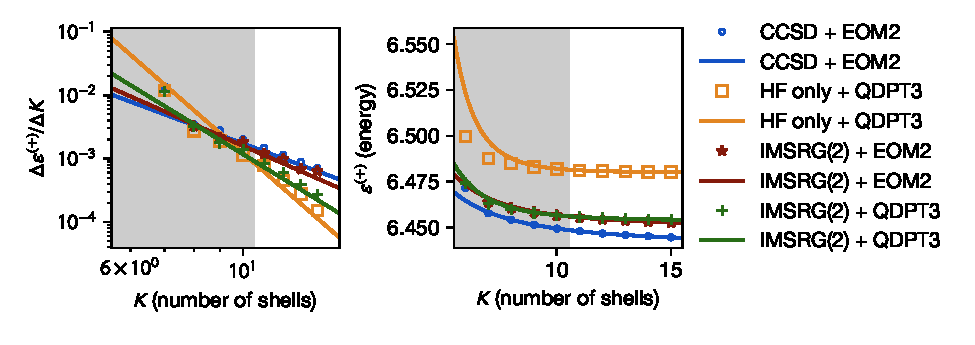
\includegraphics{fig-fit-2-1p0-add}
  \caption{A five-point fit of the addition energies of the $(N, \omega) = (6, 1.0)$ system with $K_{\text{stop}} = 15$.  The grey shaded region contains the masked data points, which are ignored by the fitting procedure.  The left figure plots the central difference of the addition energies $\varepsilon^{(+)}$ with respect to the number of shells $K$.  On such a plot, the power law model should appear as a straight line.  The fits are optimized using the procedure described in Section \ref{subsec:extrapolation}.  Note that the lines do not evenly pass through the points in the left plot as the fitting weights are tuned for the energy on a linear scale, not the energy differences on a logarithmic scale.}
  \label{fig:by-fit-2-1p0-add}
\end{figure}

As derived by Kvaal \cite{PhysRevB.80.045321,Kvaal2007}, the asymptotic convergence of the quantum dot observables in a finite harmonic oscillator basis can be approximately described by a power law model:
\begin{align*}
  \Delta E \propto K^{-\beta}
\end{align*}
where $\Delta E$ is the difference between the finite-basis result and the infinite-basis result, $K$ is the number of shells in the single-particle basis, and $\beta$ is some positive real exponent.  The \textit{smoothness} of the exact wave function determines the rate of the convergence: the more times the exact wave function can be differentiated, the higher the exponent $\beta$.

It is difficult to ascertain what $\beta$ is \textit{a priori}, thus we will empirically compute $\beta$ by fitting the following model through our data:
\begin{align} \label{eq:power_law_model}
  E = \alpha K^{-\beta} + \gamma
\end{align}
As a nonlinear curve fit, it can be quite sensitive to the initial parameters.  Therefore, good guesses of the parameters are necessary to obtain a sensible result.  For this, we first fit a linear model of $\log |\partial E / \partial K|$ against $\log K$:
\begin{align*}
  \log \left|\frac{\partial E}{\partial K}\right| = - (\beta + 1) \log K + \log|\alpha \beta|
\end{align*}
This is useful because linear fits are very robust and will often converge even if the initial parameters are complete nonsense.  It also provides a means to visually judge quality of the fit.  The derivative is approximated using the central difference:
\begin{align*}
  \frac{\partial E}{\partial K} \approx E\left(K + \frac{1}{2}\right) - E\left(K - \frac{1}{2}\right)
\end{align*}
The process of calculating a numericaly derivative can amplify the noise in the data and distorts the weights of the data points.  Moreover, it does not provide a means to compute $\gamma$, the extrapolated energy.  Thus a second accurate nonlinear curve fit is necessary.

The parameters $\alpha$ and $\beta$ are extracted from the linear fit and used as inputs for a power-law fit of $E$ against $K$.  It necessary to estimate the infinite-basis energy $\gamma$ as well, which is done by fitting \eqref{eq:power_law_model} while the parameters $\alpha$ and $\beta$ are fixed to the initial guesses.  The fixing ensures that the fit is still linear in nature and thus highly likely to converge.  Afterward, we do a final fit with all three parameters free to vary.  All fits are done using the traditional Levenberg--Marquardt (LM) optimization algorithm as implemented in \texttt{Minpack}, with equal weighting of all data points.

There is still one additional tuning knob for this model that is not explicitly part of \eqref{eq:power_law_model}: the range of data points taken into consideration (\textit{fit range}).  Since the model describes the \emph{asymptotic} behavior, we do not expect the fit to produce good results when the energy is still very far from convergence.  To account for this, we only fit the last few data points within some chosen range.  If range is too large, then the non-asymptotic behavior would perturb the result too much, whereas if the range is too small, there would be more noise and less confidence in whether the trend is legitimate rather than accidental.  Empirically, we chose to fit the last 5 points of our available data.  The results are shown in Tables \ref{tab:ground-extrapolated}, \ref{tab:add-extrapolated}, and \ref{tab:rm-extrapolated}.  A specific example of the fit is shown in Figure \ref{fig:by-fit-2-1p0-add}

The LM fitting procedure also computes uncertainties for the parameters from an approximate Hessian of the model function.  It is therefore tempting to use the uncertainty of the fit to quantify the uncertainty of the extrapolated energy.  We certainly would not expect this to account for the error due to the operator truncation, but how accurately does it quantify the discrepancy of our extrapolated result from the true infinite-basis energy?

We investigated this idea by performing a fit over \emph{all possible} 5-point fit ranges $[K_{\text{stop}} - 4, K_{\text{stop}}]$.  By comparing the extrapolated results at varying values of $K_{\text{stop}}$ with the extrapolated result at the highest possible $K_{\text{stop}}$ and treating the latter as the ``true'' infinite-basis result, we can statistically assess whether the fit uncertainties are a good measure of the discrepancy from the true infinite-basis result.  Our results show a somewhat bimodal distribution: when the relative fit uncertainty is higher than $10^{-3.5}$, the fit uncertainty quantifies the discrepancy well; otherwise, the fit uncertainty underestimates the discrepancy by a factor of 10 or less.

Unlike the other methods, Hartree--Fock energies are somewhat unusual in that they generally do not conform to the power-law model.  In fact, the results and plots seem to indicate an \emph{exponential} convergence with respect to the number of shells.  It is likely that HF is insensitive to the Coulomb cusp.

Nonetheless, despite the poor fits that often arise, the extrapolated energies are often quite good for HF.  This is likely due to its rapid convergence, which leaves very little degree of freedom even for a poorly chosen model.  Moreover, we found that the fit uncertainties of energy are fairly good measures of the true discrepancy.

Not all fits yield a positive value of $\beta$ for addition and removal energies, which suggests that the data points do not converge, or require a very high number of shells to converge.  These cases are marked ``n.f.'' in the tables.  This affects exclusively IM-SRG(2) + QDPT3 for systems with few particles and low frequencies, indicating that perturbation theory is inadequate for such systems.

\section{Conclusions}
\label{sec:conclusions}

We have demonstrated calculations of ground state, addition, and removal energies of two-dimensional circular quantum dots using a variety of many-body methods: ranging from the basic Hartree-Fock method, to more sophisticated combinations of IM-SRG, CC, QDPT and/or EOM.  Many closed-shell quantum dot systems have been explored, ranging from 2 to 56 particles and frequencies between 0.1 and 1.0.  All such results show good agreement with one another.

We note that the HF + IM-SRG + QDPT combination provides a reasonable moderate-cost approach to the calculation of addition and removal energies for many systems in comparison to the somewhat more expensive and complicated EOM calculations.  Both IM-SRG and CC are reasonably accurate compared to the near-exact but factorial-cost FCI method, allowing exploration of much higher number of particles than would otherwise be possible.  EOM-IM-SRG does have more flexibility over perturbative approaches: in particular, it could be more readily used to construct excited states \cite{2016arXiv161100661P}, which is more difficult for methods such as DMC.

There are several directions in which the calculations may be improved.  One can attempt to improve the IM-SRG approximation by incorporating some of the missing higher-body terms in the commutator.  This would also provide some insight into the rate of convergence with respect to the operator truncation, providing a sense of how large the truncation error is.  While a full 3-body treatment of IM-SRG would be extremely costly, it is possible implicitly track for a portion of the induced 3-body forces by computing certain diagrams that are either lower cost or could be approximated at lower cost \cite{IMSRG}.

The application of IM-SRG eliminates a large number of the QDPT diagrams \ref{fig:diagrams-sfe}, which is beneficial as it increases the efficiency of the QDPT calculations.  Thus it may be more feasible to perform higher orders of QDPT on IM-SRG evolved Hamiltonians.  Moreover, the remaining diagrams at third order can be eliminated through infinite resummation techniques, which would incorporate higher order terms and therefore further increase the accuracy of the result.

We note that this calculation was done entirely using the traditional approach of using a high-order ODE solver to solve the flow equation.  A new technique developed by T. D. Morris \cite{PhysRevC.92.034331} uses an alternative approach that obviates the need for a high-order ODE solver, leading to much more efficient computations and also allowing operators of other observables to be evolved at lower cost, which poses a significant advantage over coupled cluster methods.  Implementing this approach would allows us to study the accuracy and convergence of other possibly more sensitive observables.

The IM-SRG method can be extended to support multiple reference states (multi-reference IM-SRG or simply MR-IM-SRG) \cite{PhysRevLett.110.242501,PhysRevC.90.041302} through the generalized normal ordering formalisms \cite{doi:10.1063/1.474405}, which opens the possibility of calculating quantum systems that are far from the magic numbers (open-shell systems).  This is a territory that few many-body methods can tackle and is one of the major strengths of the IM-SRG approach.

By transforming of the operator-SRG rather than the wave function, IM-SRG is more amenable to the construction of softened \textit{effective interactions} than CC \cite{Hergert2016165}.  Such interactions can be used to lower the cost of other methods such as configuration interaction (CI), also known as \textit{shell model} in nuclear physics.

Implementation-wise, our current code constructs the two-particle states as simple Slater determinants of their one-particle states.  This approach is often referred to as \textit{m-scheme} in nuclear physics.  It is straightforward to implement and works well for general systems, but it fails to exploit all the symmetries in the quantum dot system: not only is spin projection $\hat S_z$ conserved, the Casimir operator $\hat S^2$ is as well.  A more efficient approach is to couple the spins of the single-particle states to form two-particle states with good $\hat S^2$, an approach analogous to \textit{j-scheme} in nuclear physics.  A combination of this with the Eckart-Wigner theorem could reduce the computational cost significantly, albeit at the cost of increased implementation complexity.

Currently, parallelism within the code is limited to a thread level, i.e.\ shared memory parallelism: the program does cannot take advantage of more than a single compute node, thus it would not scale well on modern high-performance computing facilities.  Rewriting the algorithm to take advantage of distributed memory parallelism would allow the workload and memory resources to be divided over many computing nodes, allowing larger systems to be explored.  As with any parallelization, the algorithm must be designed carefully to minimize the communication, which are significantly more costly in parallel platforms.

We hope to apply these theoretical and technical enhancements not only to the study of quantum dots, but to studies of nuclear and atomic systems, opening up an even greater range of applications.

\begin{acknowledgments}
  This work was supported by the National Science Foundation Grant No.\ PHY-1404159 (Michigan State University) and by the Research Council of Norway under contract ISP-Fysikk/216699.  This research used computational resources of the Notur project in Norway.  We thank Christoffer Hirth, Simen Kvaal and Veronica Olsen for several discussions.
\end{acknowledgments}

\bibliographystyle{\mybibstyle}
\bibliography{paper}
\end{document}
